%%%%%%%%%%%%%%%%%%%%%%%%%%%%%%%%%%%%%%%%%%%%%%%%%%%%%%%%%%%%%%%
% Document Class Configuration
%%%%%%%%%%%%%%%%%%%%%%%%%%%%%%%%%%%%%%%%%%%%%%%%%%%%%%%%%%%%%%%
\documentclass[openany]{book}

%%%%%%%%%%%%%%%%%%%%%%%%%%%%%%%%%%%%%%%%%%%%%%%%%%%%%%%%%%%%%%%
% Basic Packages
%%%%%%%%%%%%%%%%%%%%%%%%%%%%%%%%%%%%%%%%%%%%%%%%%%%%%%%%%%%%%%%
% Language settings
\usepackage[english]{babel}

% Page geometry and layout
\usepackage{geometry}
\geometry{
    a4paper,           % Paper size
    total={170mm,237mm}, % Total usable area
    left=20mm,         % Left margin
    top=30mm          % Top margin
}

% Line spacing control
\usepackage{setspace}
\onehalfspacing       % Set 1.5 line spacing for the document

%%%%%%%%%%%%%%%%%%%%%%%%%%%%%%%%%%%%%%%%%%%%%%%%%%%%%%%%%%%%%%%
% Mathematical Packages and Settings
%%%%%%%%%%%%%%%%%%%%%%%%%%%%%%%%%%%%%%%%%%%%%%%%%%%%%%%%%%%%%%%
\usepackage{
    amsmath,    % Advanced math formatting
    amsthm,     % Theorem environments
    amsfonts,   % Mathematical fonts
    bm          % Bold math symbols
}

%%%%%%%%%%%%%%%%%%%%%%%%%%%%%%%%%%%%%%%%%%%%%%%%%%%%%%%%%%%%%%%
% Graphics and Figures
%%%%%%%%%%%%%%%%%%%%%%%%%%%%%%%%%%%%%%%%%%%%%%%%%%%%%%%%%%%%%%%
\usepackage{graphicx}  % Include graphics
\usepackage{float}     % Improved float environment
\usepackage{tikz}      % Drawing tools
\graphicspath{{./images/}}  % Path for images

%%%%%%%%%%%%%%%%%%%%%%%%%%%%%%%%%%%%%%%%%%%%%%%%%%%%%%%%%%%%%%%
% Header, Footer, and Hyperlinks
%%%%%%%%%%%%%%%%%%%%%%%%%%%%%%%%%%%%%%%%%%%%%%%%%%%%%%%%%%%%%%%
\usepackage[hidelinks]{hyperref}  % Hyperlinks without colored borders
\usepackage{fancyhdr}             % Custom headers and footers

% Header and footer configuration
\pagestyle{fancy}
\fancyhf{}                        % Clear all header/footer fields
\renewcommand{\headrulewidth}{0pt}% Remove header rule
\fancyfoot[C]{\thepage}          % Center page number in footer
\setlength{\footskip}{50pt}      % Footer distance from text

%%%%%%%%%%%%%%%%%%%%%%%%%%%%%%%%%%%%%%%%%%%%%%%%%%%%%%%%%%%%%%%
% Custom Mathematical Operators and Commands
%%%%%%%%%%%%%%%%%%%%%%%%%%%%%%%%%%%%%%%%%%%%%%%%%%%%%%%%%%%%%%%
% Function evaluation
\newcommand\at[2]{\left.#1\right|_{#2}}

% Mathematical operators
\DeclareMathOperator{\sgn}{sgn}           % Sign function
\DeclareMathOperator{\col}{col}           % Column operator
\DeclareMathOperator{\des}{des}           % Descent operator
\DeclareMathOperator*{\argmax}{arg\,max}  % Argument of maximum
\DeclareMathOperator*{\argmin}{arg\,min}  % Argument of minimum

% Special symbols and notations
\newcommand{\notimplies}{%
    \mathrel{{\ooalign{\hidewidth$\not\phantom{=}$\hidewidth\cr$\implies$}}}}
\newcommand{\R}{\mathbb{R}}               % Real numbers
\newcommand{\N}{\mathbb{N}}               % Natural numbers
\newcommand{\deriv}[1]{\displaystyle\frac{d}{d #1}}  % Derivative
\newcommand{\traj}{(\bar{\mathbf{x}},\bar{\mathbf{u}})}  % Trajectory

%%%%%%%%%%%%%%%%%%%%%%%%%%%%%%%%%%%%%%%%%%%%%%%%%%%%%%%%%%%%%%%
% Theorem Environments
%%%%%%%%%%%%%%%%%%%%%%%%%%%%%%%%%%%%%%%%%%%%%%%%%%%%%%%%%%%%%%%
% Definition-style theorems
\theoremstyle{definition}
\newtheorem{definition}{Definition}[section]
\newtheorem{theorem}{Theorem}[section]
\newtheorem{proposition}{Proposition}[section]
\newtheorem*{corollary}{Corollary}

% Remark-style theorems
\theoremstyle{remark}
\newtheorem*{remark}{Remark}
\newtheorem*{notation}{Notation}

%%%%%%%%%%%%%%%%%%%%%%%%%%%%%%%%%%%%%%%%%%%%%%%%%%%%%%%%%%%%%%%
% Document Information
%%%%%%%%%%%%%%%%%%%%%%%%%%%%%%%%%%%%%%%%%%%%%%%%%%%%%%%%%%%%%%%
\title{Optimal Control M}
\author{Giorgio Medico based on Dante Piotto's notes}
\date{fall semester 2024}


\begin{document}
\maketitle
\tableofcontents

\chapter*{Course Overview}
This course focuses on optimization-based control of dynamical systems. It provides theoretical and numerical methods to compute control system trajectories that minimize a performance index, with particular emphasis on their application to trajectory optimization and maneuvering of Autonomous Systems.

\section*{Learning Objectives}
Upon completion of this course, students will be able to:
\begin{enumerate}
    \item Set up optimal control problems and characterize optimality conditions
    \item Develop numerical optimization methods to compute optimal, feasible trajectories
    \item Design optimization-based receding-horizon control schemes for nonlinear systems
\end{enumerate}

\section*{Course Applications}
To bridge the gap between theory and application, students will apply the proposed techniques to trajectory optimization and maneuvering of Autonomous Systems across various domains including:
\begin{itemize}
    \item Autonomous Vehicles
    \item Robotic Systems (e.g., Aerial Robots)
    \item Other Mechatronic Systems
\end{itemize}

\chapter{Introduction to optimal control}

\section{Optimal control problem formulation}
Consider the continuous-time system (State-Space representation) ($t\in\R$)

\begin{equation}\label{system}
    \begin{gathered}\
        \dot{x}(t) = f(x(t),u(t),t) \\
        y(t) = h(x(t),u(t),t)
    \end{gathered}
\end{equation}

\begin{itemize}
    \item $x(t)\in\R^n$ state of the system at time $t$ 
    \item $u(t)\in\R^m$ input of the system at time $t$ 
    \item $y(t)\in\R^p$ output of the system at time $t$
\end{itemize}
We will mainly work with time invariant systems, $\dot{x}(t)=f(x(t),u(t))$. \\[0.5cm]
We consider nonlinear, discrete-time systems described by Finite-Difference Equations (FDE):
\[
    x(t+1)=f_t(x(t),u(t)) \quad t\in\N_0
\]
but from now on we will use the compact notation
\[
    x_{t+1}=f_t(x_t,u_t) \quad t\in\N_0
\]
where $x_t\in\R^n$ and $u_t\in\R^m$ are the state and the input of the system at time $t$.

Consider a nonlinear, discrete-time system on a finite time horizon 
\[
    x_{t+1} = f_t(x_t,u_t) \quad t=0,\dots,T-1
\]
We use $\mathbf{x}\in\R^{nT}$ and $\mathbf{u}\in\R^{mT}$ to denote, respectively, the stack of the states $x_t$ for all $t\in\{1,\dots,T\}$ and the inputs $u_t$ for all $t\in\{0,\dots,T-1\}$, that is:
\begin{gather*}
    \mathbf{x} := \begin{bmatrix}
        x_1 \\ \vdots \\ x_T
    \end{bmatrix} \qquad
    \mathbf{u} := \begin{bmatrix}
        u_0 \\ \vdots \\ u_{T-1}
    \end{bmatrix}
\end{gather*}

\subsubsection{Trajectory of a system}

\textbf{Definition:} A pair ($\bar{\mathbf{x}},\bar{\mathbf{u}})\in\R^{nT} \times \R^{mT}$ is called a trajectory of system \eqref{system} 
if $\bar{x}_{t+1}=f_t(\bar{x}_t,\bar{u}_t)$ for all $t\in\{0,\dots,T-1\}$. That is, if $(\bar{\mathbf{x}},\bar{\mathbf{u}})$ satisfies the system dynamics (the same holds for continuous time systems with proper adjustments). In particular, $\bar{\mathbf{x}}$ is the state trajectory, while $\bar{\mathbf{u}}$ is the input trajectory.

\subsubsection{Equilibrium}

\textbf{Definition:} A state-input pair $(x_e,u_e)\in\R^n\times\R^m$ is called an equilibrium pair of \eqref{system} if $(x_t,u_t)=(x_e,u_e),\forall t\in\N_0$ is a trajectory of the system. Equilibria of time-invariant systems satisfy $x_e=f(x_e,u_e)$

\subsubsection{Linearization of a system about a trajectory}
Given the dynamics \eqref{system}
and a trajectory $(\bar{\mathbf{x}},\bar{\mathbf{u}})$, the linearization of \eqref{system} about $(\bar{\mathbf{x}},\bar{\mathbf{u}})$ is given by the linear (possibly) time-varying system 
\[
    \Delta x_{t+1} = A_t\Delta x_t + B_t \Delta u_t \quad t\in\N_0
\]
with $A_t$ and $B_t$ the Jacobians of $f_t$, with respect to state and input respectively, evaluated at $(\bar{\mathbf{x}},\bar{\mathbf{u}})$
\[
    A_t = \at{\displaystyle\frac{\partial}{\partial x}f(\bar{x}_t,\bar{u}_t)}{(\bar{\mathbf{x}},\bar{\mathbf{u}})} \quad B_t = \at{\displaystyle\frac{\partial}{\partial u}f(\bar{x}_t,\bar{u}_t)}{(\bar{\mathbf{x}},\bar{\mathbf{u}})}
\]
where $x_t \approx \bar{x}_t + \Delta x_t$ and $u_t \approx \bar{u}_t + \Delta u_t$.\\ 
($\bar{x_t}$ and $\bar{u_t}$ are the nominal trajectory values of $x_{t+1} = f_t(x_t,u_t)$ and $\Delta x_t$, $\Delta u_t$ are the trajectory of the linearized system.)


\subsection{Optimization}
\subsubsection{Main ingredients}
\begin{itemize}
    \item Decision variable: $z\in\R^d$ 
    \item Cost function: $\ell(z):\R^d\to\R$ cost associated to decision $z$
    \item Constraints (constraint sets): for some given functions $h_i:\R^d\to\R,  \text{ and } g_j:\R^d\to\R,$ the decision vector $z\in\R^d$ needs to satisfy 
        \begin{gather*}
            h_i(z)=0 \quad i=1,\dots,m \\
            g_j(z)\leq0 \quad j=1,\dots,r
        \end{gather*}
        equivalently we can say that we require $z\in Z$ with 
        \[
            Z=\{z\in\R^d|h(z)=0, g(z)\leq 0\},
        \]
        where we compactly denoted $h(z)=\col(h_1(z),\dots,h_m(z))$ and $g(z) = \col(g_1(z),\dots,g_r(z))$
\end{itemize}

\subsubsection{Minimization}
We can write our optimization problem as 
\begin{align*}
    \min_{z\in\R^d} &\ell(z)\\
    \text{subj. to } &h_i(z) = 0 \quad i=1,\dots,m\\
    &g_j(z)\leq 0 \quad j=1,\dots,r
\end{align*}
where $h_i:\R^d\to\R$ and $g_j:\R^d\to\R$\\
We can write it more compactly as 
\begin{align*}
    \min_{z\in\R^d} &\ell(z)\\
    \text{subj. to } &h(z) = 0 \\
    &g(z)\leq 0 
\end{align*}
where $h:\R^d\to\R^m$ and $g:\R^d\to\R^r$
\subsection{Discrete-time optimal control}
\subsubsection{Main Ingredients}
\begin{itemize}
    \item Dynamics: a discrete-time system in state space form 
        \[
            x_{t+1} = f_t(x_t,u_t) \quad t=0,1,\dots,T-1
        \]
    \item the dynamics introduce $T$ equality constraints 
        \[
            \begin{array}{l l l}
                x_1 = f(x_0,u_0) & \quad \text{i.e.} \quad& x_1-f_t(x_0,u_0)=0 \\
                x_2 = f(x_1,u_1) & \quad \text{i.e.} \quad & x_2-f_t(x_1,u_1)=0 \\
                \vdots \\
                x_T = f(x_{T-1},u_{T-1}) & \quad \text{i.e.} \quad & x_T-f_t(x_{T-1},u_{T-1})=0 \\
            \end{array}
        \] 
        This is equivalent to $nT$ scalar constraints
    \item Cost function: a cost "to be payed" for a chosen trajectory. We consider an additive structure in time 
        \[
            \ell(\mathbf{x},\mathbf{u}) = \displaystyle\sum_{t=0}^{T-1}\ell_t(x_t,u_t)+\ell_T(x_T)
        \]
        where $\ell_t:\R^n\times\R^m\to\R$ is called stage-cost, while $\ell_T:\R^n\to\R$ is the terminal cost. 
    \item End-point constraints: function of the state variable prescribed at initial and/or final point 
        \[
            r(x_0,x_T)=0
        \]
    \item Path constraints: point-wise (in time) constraints representing possible limits on states and inputs at each time $t$ 
        \[
            g_t(x_t,u_t)\leq 0, \quad t\in\{0,\dots,T-1\}
        \]
\end{itemize}


A discrete-time optimal control problem can be written as 
\begin{gather*}
    \min_{\substack{x_0,x_1,\dots,x_T\\u_0,\dots,u_{T-1}}} \displaystyle\sum_{t=0}^{T-1}\ell_t(x_t,u_t)+\ell_T(x_T)\\[10pt]
    \begin{array}{l l }
        \text{subj. to } & x_{t+1}=f_t(x_t,u_t), \quad t\in\{0,\dots,T-1\}\\[5pt]
                         & r(x_0,x_T) = 0  \\[5pt]
                         & g_t(x_t,u_t)\leq 0, \quad t\in\{0,\dots,T-1\}
    \end{array}
\end{gather*}

\subsubsection{Optimal control for trajectory generation}
We can pose a trajectory generation problem as 
\begin{gather*}
    \min_{\mathbf{x}\in\R^n,\mathbf{u}\in\R^m}\displaystyle\sum_{t=0}^{T-1}\displaystyle\frac{1}{2}\|x_t-x_t^{\des}\|^2_Q + \displaystyle\frac{1}{2}\|u_t-u_t^{\des}\|^2_R + \displaystyle\frac{1}{2}\|x_T-x_T^{\des}\|^2_{P_f}
\end{gather*}

\subsubsection{Continuous-time Optimal Control problem}
A continuous-time optimal control problem, i.e., $t\in\R$ can be written as 
\begin{gather*}
    \min_{(x(\cdot),u(\cdot))\in \mathcal{F}}\displaystyle\int_{0}^{T}\ell_\tau(x(\tau),u(\tau))d\tau+\ell_T(x(T))\\
    \begin{array}{l l}
        \text{subj. to } & \dot{x}(t) = f_t(x(t),u(t)) \quad t\in[0,T]\\
                         & r(x(0),x(T)) = 0 \\
                         & g_t(x(t),u(t))\leq 0 \quad t\in[0,T)
    \end{array}
\end{gather*}
Note that $\mathcal{F}$ is a space of functions (function space). This is an infinite dimensional optimization problem
\begin{itemize}
    \item Cost functional $\ell:\mathcal{F}\to\R$
        \[
            \ell(x(\cdot),u(\cdot)) = \displaystyle\int_{0}^{T}\ell_\tau(x(\tau),u(\tau))d\tau+\ell_T(x(T))
        \]
    \item Space of trajectories (or trajectory manifold)
        \[
            \mathcal{T} = \{(x(\cdot),u(\cdot))\in\mathcal{F}\ |\ \dot{x}(t)=f_t(x(t),u(t)),\ t\geq 0\}
        \]
\end{itemize}

\chapter{Nonlinear Optimization}

\section{Overview}

\begin{enumerate}
    \item \textbf{Motivating Examples}
        \begin{itemize}
            \item Drone trajectory generation
            \item Pendulum control
            \item Trajectory manifold concept
        \end{itemize}
    
    \item \textbf{Theoretical Foundations}
        \begin{itemize}
            \item Types of minima
                \begin{itemize}
                    \item Global/Local
                    \item Strict/Non-strict
                \end{itemize}
            \item Optimality conditions
                \begin{itemize}
                    \item First-order necessary
                    \item Second-order necessary
                    \item Second-order sufficient
                \end{itemize}
        \end{itemize}
    
    \item \textbf{Convex Optimization}
        \begin{itemize}
            \item Convex sets and functions
            \item Constraint definitions
            \item Properties
                \begin{itemize}
                    \item Local = Global minima
                    \item First-order sufficiency
                \end{itemize}
            \item Quadratic programs
        \end{itemize}
    
    \item \textbf{Solution Methods}
        \begin{itemize}
            \item Iterative descent methods
                \begin{itemize}
                    \item Gradient methods
                    \item Quadratic minimization
                \end{itemize}
            \item Newton's method
                \begin{itemize}
                    \item Zero-finding
                    \item Unconstrained optimization
                \end{itemize}
            \item Step-size selection
                \begin{itemize}
                    \item Constant
                    \item Diminishing
                    \item Armijo rule
                \end{itemize}
        \end{itemize}
    
    \item \textbf{Constrained Optimization}
        \begin{itemize}
            \item Convex set optimization
                \begin{itemize}
                    \item Projection methods
                    \item Feasible directions
                \end{itemize}
            \item Equality/Inequality constraints
                \begin{itemize}
                    \item Active constraints
                    \item KKT conditions
                    \item Complementary slackness
                \end{itemize}
            \item Advanced methods
                \begin{itemize}
                    \item Sequential Quadratic Programming
                    \item Barrier functions
                \end{itemize}
        \end{itemize}
    
    \item \textbf{Implementation}
        \begin{itemize}
            \item Python implementation
            \item Convergence visualization
            \item Performance analysis
        \end{itemize}
\end{enumerate}

\textbf{Nonlinear programming (NLP) is the process of solving an optimization problem where the objective function or some of the constraints are Non-Linear.}

\section{Unconstrained Optimization}
Consider the unconstrained optimization problem 
\[
    \min_{z\in\R^n}\ell(z)
\]
with $\ell:\R^d\to\R$ a cost function to be minimized and $z$ a decision vector 

We say that $z^*$ is a  
\begin{itemize}
    \item global minimum if $\ell(z^*)\leq\ell(z)$ for all $z\in\R^n$ 
    \item strict global minimum if $\ell(z^*)<\ell(z)$ for all $z\neq z^*$
    \item local minimum if there exists $\epsilon>0$ such that $\ell(z^*)\leq\ell(z)$ for all $z\in B(z^*,\epsilon) = \{z\in\R^d| \|z-z^*\|<\epsilon\}$
    \item strict local minimum if there exists $\epsilon>0$ such that $\ell(z^*)<\ell(z)$ for all $z\in B(z^*,\epsilon)$ 

\end{itemize}

\begin{figure}[ht]
    \centering
    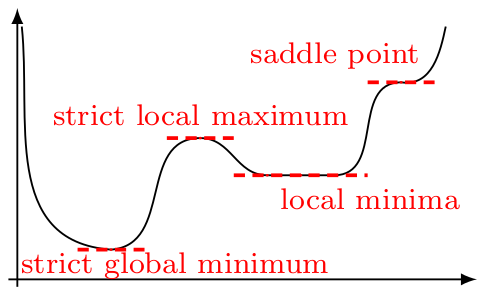
\includegraphics[width=0.35\textwidth]{min.png}
    \caption{Illustration of different types of minima in an optimization problem}
    \label{fig:min}
\end{figure}

\subsubsection{Notation}
We denote $\ell(z^*)$ the optimal (minimum) value of a generic optimization problem, i.e. 
\[
    \ell(z^*) = \min_{z\in\R^d}\ell(z)
\]
where $z^*$ is the minimum point (optimal value for the optimization variable) i.e. 
\[
    z^* = \argmin_{z\in\R^d} \ell(z)
\]
\subsubsection{Gradient and Hessian}
Gradient of a function: for a function $r:\R^d\to\R$  the gradient is denoted as 
\[
    \nabla r(z) = \begin{bmatrix}
        \displaystyle\frac{\partial r(z)}{\partial z_1} \\ \vdots \\ \displaystyle\frac{\partial r(z)}{\partial z_d}
    \end{bmatrix} \in \R^{d\times 1}
\]
Hessian matrix of a function: for a function $r:\R^d\to\R$  the Hessian matrix is denoted as 
\[
    \nabla^2(r(z)) = \begin{bmatrix}
        \displaystyle\frac{\partial^2 r(z)}{\partial z_1^2} & \cdots & \displaystyle\frac{\partial^2 r(z)}{\partial z_1z_d} \\ \vdots & \ddots & \vdots \\ \displaystyle\frac{\partial^2 r(z)}{\partial z_dz_1} & \cdots & \displaystyle\frac{\partial^2 r(z)}{\partial z_d^2}
    \end{bmatrix} \in \R^{d\times d}
\]
The Hessian matrix is a symmetric matrix, since the assumption of continuity of the second derivatives implies that the order of differentiation does not matter.\\

Gradient of a vector-valued function: for a vector field $r:\R^d\to\R^m$, the gradient is denoted as 
\[
    \nabla r(z) = \begin{bmatrix}
        \nabla r_1(z) & \cdots & \nabla r_m(z)
    \end{bmatrix} = \begin{bmatrix}
        \displaystyle\frac{\partial r_1(z)}{\partial z_1} & \cdots & \displaystyle\frac{\partial r_m(z)}{\partial z_1} \\
        \vdots & \ddots & \vdots \\
        \displaystyle\frac{\partial r_1(z)}{\partial z_d} & \cdots & \displaystyle\frac{\partial r_m(z)}{\partial z_d} \\
    \end{bmatrix} \in \R^{d\times m}
\]
which is the transpose of the Jacobian matrix of $r$

\subsection{Conditions of optimality}

\subsubsection{First order Necessary condition (FNC) of optimality (unconstrained)}

Let $z^*$ be an unconstrained local minimum of $\ell:\R^d\to\R$ and assume that $\ell$ is continuously differentiable ($\mathcal{C}^1$) in $B(z^*,\varepsilon)$\footnote{Ball of radius $\varepsilon$ centered in $z^*$} for some $\varepsilon>0$. Then $\nabla \ell(z^*)=0$ (the gradient of $\ell$ at $z^*$ is zero).

\subsubsection{Second order Necessary condition (FNC) of optimality (unconstrained)}

If additionally $\ell$ is twice continuously differentiable ($\mathcal{C}^2$) in $B(z^*,\varepsilon)$, then $\nabla^2 \ell(z^*)\geq 0$ (The Hessian of $\ell$ is positive semidifinite).
\\
% Remark 
\begin{remark}
    Points $\bar{z}$ satisfying $\nabla \ell(\bar{z})=0$ are called stationary points. They include minima, maxima and
saddle points.
\end{remark}

\subsubsection{Second order Sufficient conditions of optimality (unconstrained)}

Let $\ell:\R^d\to\R\in\mathcal{C}^2$ (twice differentiable) in $B(z^*,\varepsilon)$ for some $\varepsilon>0$. Suppose that $z^*\in\R^d$ satisfies 
\[
    \nabla\ell(z^*) = 0\quad \text{and} \quad \nabla^2\ell(z^*)>0
\]
Then $z^*$ is a strict (unconstrained) local minimum of $\ell$

\subsubsection{Convex set} 
A set $Z\subset \R^d$ is convex if for any two points $z_A$ and $z_B$ in $Z$ and for all $\theta\in[0,1]$, then 
\[
    \theta z_A + (1-\theta)z_B \in Z
\]
\begin{figure}[ht]
    \centering
    \begin{minipage}{.5\textwidth}
        \centering
        \includegraphics[width=0.3\linewidth]{cvxset}
    \caption{Convex set}
    \end{minipage}%
    \begin{minipage}{.5\textwidth}
        \centering
        \includegraphics[width=0.3\linewidth]{ncvxset}
    \caption{Non convex set}
    \end{minipage}
\end{figure}

\subsubsection{Convex functions}
Let $Z \subset \R^d$ be a convex set. A function $\ell:Z\to\R$ is convex if for any two points $z_A$ and $z_B$ in $Z$ and for all $\theta\in[0,1]$, then 
\[
    \ell(\theta z_A + (1-\theta)z_B)\leq \theta\ell(z_A)+ (1-\theta)\ell(z_B)
\]
\begin{figure}[ht]
    \centering
    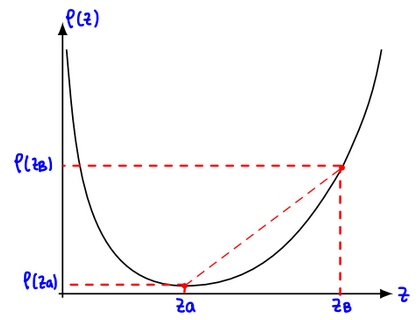
\includegraphics[width=0.3\textwidth]{cvxfcn}
    \caption{Convex function}
\end{figure}

\begin{remark}
A function $\ell$ is \emph{concave} if $-\ell$ is convex. A function $\ell$ is strictly convex if the inequality holds strictly for $z_A\neq z_B$ and $\theta\in(0,1)$.
\end{remark}

\subsubsection{Inequality constraints and convex sets}
Let $g:\R^d\to\R^p$, we can define a set $Z_{\text{ineq}}\subset \R^d$ as
\[
    Z_{\text{ineq}} = \{z\in\R^d|g(z)\leq 0\}
\]
The set $Z_{\text{ineq}}$ is convex iff $g$ is a quasi-convex function (e.g., monotone functions on the axis)

\begin{corollary}
    if $g$ is convex then $Z_{\text{ineq}}$ is convex and vice versa.
\end{corollary}

% add const.png
\begin{figure}[ht]
    \centering
    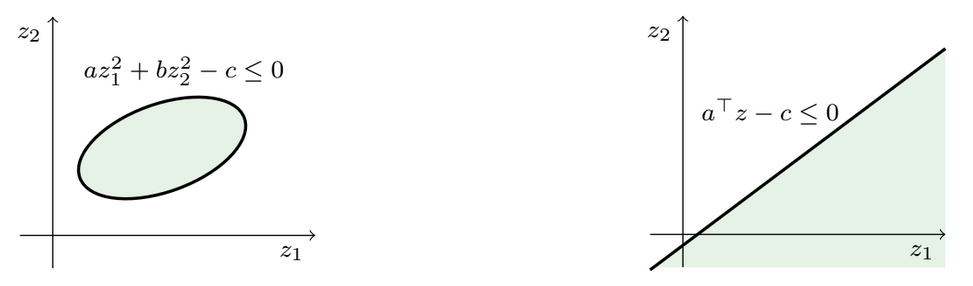
\includegraphics[width=0.7\textwidth]{const}
    \caption{Convex set identified through inequality constraints}
\end{figure}

\subsubsection{Equality constraints and convex sets}
Let $h:\R^d\to\R^p$, we can define a set $Z_{\text{eq}}\subset \R^d$ as
\[
    Z_{\text{eq}} = \{z\in\R^d|h(z)= 0\}
\]
The set $Z_{\text{eq}}$ is convex iff $h$ is an affine function. Convex sets identified through equality constraints are linear spaces (hyperplanes).

\subsubsection{Convexity and gradient monotonicity}
If $\ell$ is differentiable and convex, then for all $z_A, z_B \in Z$ it holds
\[
    \ell(z_B) \geq \ell(z_A) + \nabla\ell(z_A)^T(z_B - z_A)
\]

If $\ell$ is differentiable and convex, then its gradient $\nabla\ell: \mathbb{R}^d \to \mathbb{R}^d$ satisfies
\[
    (\nabla\ell(z_A) - \nabla\ell(z_B))^T(z_A - z_B) \geq 0
\]
for all $z_A, z_B$. That is, the gradient $\nabla\ell$ is a monotone operator.

\subsubsection{Strict convexity and gradient monotonicity}
A function $\ell$ is strictly convex if for $z_A \neq z_B$ and $\theta \in (0,1)$
\[
    \ell(\theta z_A + (1-\theta)z_B) < \theta\ell(z_A) + (1-\theta)\ell(z_B)
\]

If the strictly convex function $\ell$ is also differentiable, then its gradient satisfies
\[
    (\nabla\ell(z_A) - \nabla\ell(z_B))^T(z_A - z_B) > 0
\]
for all $z_A, z_B$. That is, the gradient $\nabla\ell$ is a strictly monotone operator.

\subsubsection{Strong convexity and gradient monotonicity}
A function $\ell$ is strongly convex with parameter $\mu > 0$ if for $z_A \neq z_B$ and $\theta \in (0,1)$
\[
    \ell(\theta z_A + (1-\theta)z_B) < \theta\ell(z_A) + (1-\theta)\ell(z_B) - \mu\theta(1-\theta)\|z_A - z_B\|^2
\]

The gradient of a differentiable strongly convex function satisfies
\[
    (\nabla\ell(z_A) - \nabla\ell(z_B))^T(z_A - z_B) \geq \mu\|z_A - z_B\|^2
\]
for all $z_A, z_B$. That is, the gradient $\nabla\ell$ is a strongly monotone operator.

\subsubsection{Convexity and Lipschitz continuity of the gradient}
Consider a differentiable convex function $\ell$ with a Lipschitz continuous gradient with parameter $L > 0$, i.e.,
\[
    \|\nabla\ell(z_A) - \nabla\ell(z_B)\| \leq L\|z_A - z_B\|
\]
for all $z_A, z_B$.

Then, the following characterization holds
\[
    (\nabla\ell(z_A) - \nabla\ell(z_B))^T(z_A - z_B) \geq \frac{1}{L}\|\nabla\ell(z_A) - \nabla\ell(z_B)\|^2
\]
for all $z_A, z_B$. That is, the gradient $\nabla\ell$ is a co-coercive operator.

\subsubsection{Strong convexity and Lipschitz continuity of the gradient}
Consider a strongly convex (with parameter $\mu > 0$) function $\ell$ with Lipschitz continuous gradient (with parameter $L > 0$)

Then the following characterization holds
\[
    (\nabla\ell(z_A) - \nabla\ell(z_B))^T(z_A - z_B) \geq \frac{\mu L}{\mu+L}\|z_A - z_B\|^2 + \frac{1}{\mu+L}\|\nabla\ell(z_A) - \nabla\ell(z_B)\|^2
\]
for all $z_A, z_B$

\subsubsection{Graphical interpretation of convexity}
If $\ell$ is differentiable and convex, then
\[
    \ell(z_B) \geq \ell(z_A) + \nabla\ell(z_A)^T(z_B - z_A)
\]
for all $z_A, z_B \in Z$

If $\ell$ is differentiable and $\mu$-strongly convex, then
\[
    \ell(z_B) \geq \ell(z_A) + \nabla\ell(z_A)^T(z_B - z_A) + \frac{\mu}{2}\|z_B - z_A\|^2
\]
for all $z_A, z_B \in Z$
\begin{figure}[ht]
    \centering
    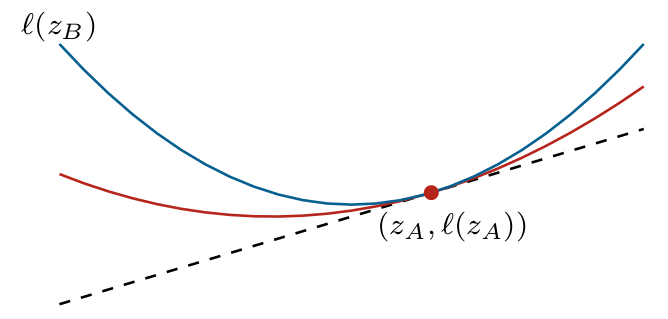
\includegraphics[width=0.4\textwidth]{quadratic lower bound on l}
    \caption{Strong convexity imposes a quadratic lower bound on $\ell$}
\end{figure}

\subsubsection{Graphical interpretation of Lipschitz continuity of the gradient}
If $\ell$ is differentiable with Lipschitz continuous gradient, then
\[
    \ell(z_B) \leq \ell(z_A) + \nabla\ell(z_A)^T(z_B - z_A) + \frac{L}{2}\|z_B - z_A\|^2
\]
for all $z_A, z_B \in Z$
\begin{figure}[ht]
    \centering
    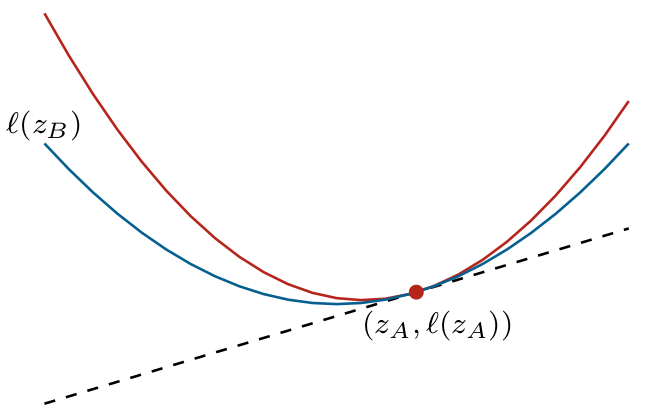
\includegraphics[width=0.4\textwidth]{quadratic upper bound on l}
    \caption{Lipschitz continuity of $\nabla\ell$ imposes a quadratic upper bound on $\ell$}
\end{figure}

\subsection{Minimization of convex functions}

\subsubsection{Proposition}
Let $Z\subset\R^d$ be a convex set and $\ell: Z\to\R$ a convex function. Then a local minimum of $\ell$ is also a global minimum. \\
Proof: not done in class but present in slides for funsies

\subsubsection{Necessary and sufficient condition of optimality (unconstrained)}
For the unconstrained minimization of a convex function it can be shown that the first order necessary condition of optimality is also sufficient (for a global minimum).

\subsubsection{Proposition}
Let $\ell:\R^d \to \R$ be a convex function. Then $z^*$ is a global minimum if and only if $\nabla\ell(z^*)=0$.\\
Proof: not done in class but present in slides for funsies

\section{Quadratic programming (unconstrained)}
Let us consider a special class of optimization problems, namely quadratic optimization problems or quadratic programs: 
\[
    \min_{z\in\R^d}z^TQz+b^Tz
\]
with $Q=Q^T\in\R^{d\times d}$ and $b\in\R^d$.


\subsubsection{Optimality conditions}
First-order necessary condition for optimality: if $z^*$ is a minimum then 
\[
    \nabla \ell(z^*)=0 \implies 2Qz^*+b=0
\]
Second-order necessary condition for optimality: if $z^*$ is a minimum then 
\[
    \nabla^2\ell(z^*)\geq 0 \implies 2Q\geq0
\]
A necessary condition for the existence of minima for a quadratic program is that $Q\geq 0$. Thus, quadratic programs admitting at least a minimum are convex optimization problems.


\subsubsection{Properties}
Since quadratic programs are convex programs ($Q\geq 0$ is necessary to have a local minimum), then the following holds: 
\begin{center}
     For a quadratic program necessary conditions of optimality are also sufficient and minima are global
\end{center}
If $Q>0$, then there exists a unique global minimum given by 
\[
    z^* = -\displaystyle\frac{1}{2}Q^{-1}b
\]

\section{Unconstrained Optimization Algorithms}
\subsection{Iterative descent methods}
We consider optimization algorithms relying on the iterative descent idea. We denote $z^k\in\R^d$ an estimate of a local minimum at iteration $k\in\N$. The algorithm starts at a given initial guess $z^0$ and iteratively generates vectors $z^1,z^2,\dots$ such that $\ell$ is decreased at each iteration, i.e. 
\[
    \ell(z^{k+1})<\ell(z^k) \qquad k = 1,2,\dots
\]
% add descent.png
\begin{figure}[ht]
    \centering
    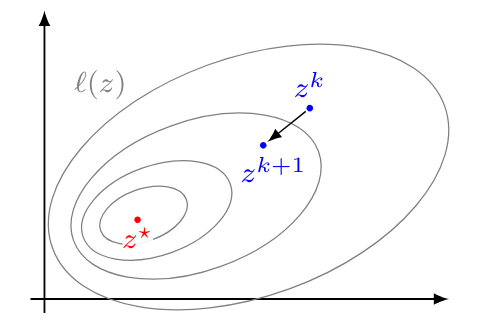
\includegraphics[width=0.35\textwidth]{descent}
    \caption{Illustration of the iterative descent idea}
\end{figure}
\subsubsection{Two-step procedure}
We consider a general two-step procedure (it's a class of algorithms) that reads as follows 
\[
    z^{k+1} = z^k+\gamma^k d^k, \qquad k=1,2,\dots
\]
in which 
\begin{enumerate}
    \item each $\gamma^k>0$ is a "step-size" 
    \item $d^k\in\R^d$ is a "direction"
\end{enumerate}
Procedure : 
\begin{enumerate}
    \item choose a direction $d^k$ along which the cost decreases for $\gamma^k$ sufficiently small;
    \item select a step-size $\gamma^k$ guaranteeing a sufficient decrease. 
\end{enumerate}
In other references these are called line-search methods.

\subsection{Gradient methods}
Let $z^k$ be such that $\nabla\ell(z^k)\neq 0$. We start by considering the update rule 
\[
    z^{k+1} = z^k-\gamma^k\nabla\ell(z^k)
\]
i.e., we choose $d^k = -\nabla\ell(z^k)$.\\
From the first order Taylor expansion of $\ell$ at $z$ we have 
\begin{align*}
    \ell(z^{k+1}) & =  \ell(z^k)+\nabla\ell(z^k)^T(z^{k+1}-z^k)+o(\|z^{k+1}-z^k\|)\\
    & =  \ell(z^k)-\gamma^k\|\nabla\ell(z^k)\|^2+o(\gamma^k)
\end{align*}
Thus, for $\gamma^k>0$ sufficiently small it can be shown that $\ell(z^k+1)<\ell(z^k)$.\\
The update rule 
\[
    z^{k+1}=z^k-\gamma^k\nabla\ell(z^k)
\]
can be generalized to so called \emph{gradient methods}
\[
    z^{k+1}=z^k+\gamma^kd^k
\]
with $d^k$ such that
\[
    \nabla\ell(z^k)^Td^k<0
\]
Also, $d^k$ must be gradient related, i.e. $d^k$ must not asymptotically become perpendicular to $\nabla\ell$

\subsubsection{Selecting the descent direction}

Several gradient methods (Generalized form) can be written as 
\[
    z^{k+1} = z^k-\gamma^kD^k\nabla\ell(z^k) \quad k=1,2,\dots
\]
where $D^k\in\R^{d\times d}$ is  a symmetric positive definite matrix. It can be immediately seen that 
\[
    -\nabla\ell(z^k)^TD^k\nabla\ell(z^k)<0
\]
i.e. $d^k = -D^k\nabla\ell(z^k)$ is a descent direction.\\
The choice of $D^k$ must be made such that there exist $d_1,d_2$ positive real, such that $d_1 I \leq D^k \leq d_2 I$.\\ [0.5cm]
Some choices for $D^k$:
\begin{itemize}
    \item Steepest descent $D^k=I_d$
    \item Newton's method $D^k = (\nabla^2\ell(z^k))^{-1}$\\
        It can be used when $\nabla^2\ell(z^k)>0$. It typically converges very fast asymptotically. For $\gamma^k = 1$ pure Newton's method
    \item Discretized Newton's method $D^k=(H(z^k))^{-1}$, where $H(z^k)$ is a positive definite symmetric approximation of $\nabla^2\ell(z^k)$ obtained by using finite difference approximations of the second derivatives 
    \item Some regularized version of the Hessian
\end{itemize}

\subsection{Steepest descent (Gradient method)}
The update rule obtained for $D^k=I$ is called steepest descent $z^{k+1} = z^k-\gamma^k\nabla\ell(z^k)$.\\
The name steepest descent is due to the following property: the normalized negative gradient direction 
\[
    d^k = -\displaystyle\frac{\nabla\ell(z^k)}{\|\nabla\ell(z^k)\|}
\]
minimizes the slope $\nabla \ell(z^k)^Td^k$ among all normalized directions, i.e. it gives the steepest descent.

\subsection{Newton's method for root(zero) finding}

Consider the nonlinear root(zero) finding problem 
\[
    r(z) = 0
\]
Idea: iteratively refine the solution such that the improved guess $z^{k+1}$ represents a root(zero) of the linear approximation of $r$ about the current tentative solution $z^k$.\\ 
Consider the linear approximation of $r$ about $z^k$, we have 
\[
    r^k(z^k+\Delta z^k) = r(z^k)+\nabla r(z^k)^T\Delta z^k
\]
then, finding the zeros of the approximation, we have
\[
    \Delta z^k = -(\nabla r(z^k)^T)^{-1}r(z^k)
\]
where $\Delta z^k = z^{k+1}-z^k$.
Thus, the solution is improved as 
\[
    z^{k+1} = z^k-(\nabla r(z^k)^T)^{-1}r(z^k)
\]

\subsection{Newton's method for Unconstrained Optimization}
Consider the unconstrained optimization problem 
\[
    \min_{z\in\R^d} \ell(z)
\]
stationary points $\bar{z}$ satisfy the first order optimality condition 
\[
    \nabla \ell (\bar{z}) = 0
\]
We can look at it as a root finding problem, with $r(z)=\nabla\ell(z)$, and solve it via Newton's method. Therefore, we can compute $\Delta z^k$ as the solution of the linearization of $r(z)=\nabla\ell(z)$ at $z^k$, i.e. 
\[
    \nabla \ell(z^k) + \nabla^2\ell(z^k)\Delta z^k = 0
\]
and run the update 
\[
    z^{k+1} = z^k -\gamma^k(\nabla^2\ell(z^k))^{-1}\nabla\ell(z^k)
\]
where in the pure Newton's method $\gamma^k=1$, in other cases $\gamma^k$ has to be selected.

\subsection{Newton's method via Quadratic Optimization}
This approach it's a way to reduce a complex problem into a sequence of simpler QP problems.
Observe that 
\[
    \nabla\ell(z^k) +\nabla^2\ell(z^k)\Delta z^k = 0
\]
is the first-order necessary and sufficient condition of optimality for the quadratic program 
\begin{equation}
    \label{qp}
    \Delta z^k = \argmin_{\Delta z}\nabla\ell(z^k)^T \Delta z+\displaystyle\frac{1}{2}\Delta z^T\nabla^2\ell(z^k)\Delta z
\end{equation}
we define $q^T = \nabla\ell(z^k)^T$ and $Q = \nabla^2\ell(z^k)$, $Q$ must be positive definite to be solvable.\\
Thus, the $k$-th iteration of Newton's method can be seen as 
\[
    z^{k+1} = z^k-\Delta z^k
\]
with $\Delta z^k$ solution of the quadratic problem \eqref{qp}. Generalized version: 
\[
    z^{k+1} = z^k - \gamma^k \Delta z^k
\]

\subsection{Gradient methods via quadratic optimization}
The "Quadratic approach" can be used with all gradient methods characterized by a certain descent direction $d^k$.
Similarly to Newton's method, a descent direction $\Delta z^k=D^k\nabla\ell(z^k)$ can be seen as the direction that minimizes at each iteration a different quadratic approximation of $\ell$ about $z^k$. 
In fact, consider the quadratic approximation $\ell^k(z)$ of $ \ell$ about $z^k$ given by the second order Taylor expansion
\[
    \ell^k(z) = \ell(z^k)+\nabla\ell(z^k)^T(z-z^k)+\displaystyle\frac{1}{2}(z-z^k)^T(D^k)^{-1}(z-z^k)
\]
By setting the derivative to zero, we have 
\[
    \nabla\ell(z^k)+(D^k)^{-1}(z-z^k)=0
\]
we can calculate the minimum of $\ell^k(z)$ and set it as the next iterate $z^{k+1}$
\[
    z^{k+1} = z^k - D^k\nabla\ell(z^k)
\]
namely, the update rule of a gradient method.
\[
    \Delta z^k = -D^k\nabla\ell(z^k)
\]
% Remark
\begin{remark}
    Direction $\Delta z^k$ can be computed by solving the quadratic approximation. This can be very
    helpful in optimization problems in which a gradient is not (easily) available, but it is to solve a quadratic
    optimization problem. It is useful also in case the domain is a compact convex set.
\end{remark}

\subsection{Step-size Selection Rules}
\begin{itemize}
    \item Constant step-size: $\gamma^k=\gamma>0$
    \item Diminishing step-size: $\gamma^k\to 0$ as $k\to\infty$. It must hold that \[
            \displaystyle\sum_{k=0}^{\infty}\gamma^k = +\infty \quad \text{and} \quad \displaystyle\sum_{k=0}^{\infty}(\gamma^k)^2 < +\infty
        \]
        The above conditions avoid pathological choices of $\gamma^k$, it must be avoided that beacons too small.
    \item Armijo rule
\end{itemize}

\subsubsection{Armijo rule}
Given the descent direction $d^k$ we can consider 
\[
    g^k(\gamma) = \ell(z^k+\gamma d^k), \quad g:\R\to\R
\]
% TODO insert image slide 30
The value of $g^k(\gamma)$ for $\gamma=0$ is $\ell(z^k)$. The minimization rule chooses as the value for $\gamma$ the value that minimizes $g^k(\gamma)$. The partial minimization rule would search for a minimum in a restricted set of values for $\gamma$. Let us differentiate $g$ wrt $\gamma$:
\begin{gather*}
    g'(\gamma)=\displaystyle\frac{d}{d\gamma}g(\gamma)=\displaystyle\frac{d}{d\gamma}\ell(z^k+\gamma d^k)\\
    g'(0) = \displaystyle\frac{d}{d\gamma}\at{\ell(z^k+\gamma d^k)}{\gamma=0} = \nabla \ell(z^k)^Td^k\\
\end{gather*}
We compute a linear approximation of $g(\gamma)$:
\begin{gather*}
    g(\gamma) = g(0) + g'(0)\gamma+o(\gamma)\\
    \ell(z^k+\gamma d^k) = \ell(z^k)+\gamma \nabla\ell(z^k)^Td^k + o(\gamma)
\end{gather*}
This is the tangent to the $g(\gamma)$ curve at $\gamma=0$. We also consider the line 
\[
    \ell(z^k)+c\gamma\nabla\ell(z^k)^Td^k
\]
which is a line with a slightly less negative slope given that $c\in(0,1)$.
The Armijo rule is applied as follows: 
\begin{enumerate}
    \item Set $\bar{\gamma}^0>0,\quad\beta\in(0,1),\quad c\in(0,1)$
    \item While $\ell(z^k+\bar{\gamma}^id^k)\geq \ell(z^k)+c\bar{\gamma}^i\nabla\ell(z^k)^Td^k$:
        \[
            \bar{\gamma}^{i+1}=\beta\bar{\gamma}^i
        \]
    \item Set $\gamma^k = \bar{\gamma}^i$
\end{enumerate}
Typical values are $\beta=0.7$ and $c=0.5$

\begin{figure}[ht]
    \centering
    \begin{minipage}{.33\textwidth}
        \centering
        \includegraphics[width=0.9\linewidth]{armijo0}
    \end{minipage}%
    \begin{minipage}{.33\textwidth}
        \centering
        \includegraphics[width=0.9\linewidth]{armijo1}
    \end{minipage}%
    \begin{minipage}{.33\textwidth}
        \centering
        \includegraphics[width=0.9\linewidth]{armijo2}
    \end{minipage}%
    \caption{The iteration stops when the $g$ function evaluated at $\gamma^k$ is below the $c$-line.}
\end{figure}

The idea is to fix the $c$-line and iterate over $\beta$ for the value of $\gamma^k$ until we obtain a value such that the $g$ function evaluated at that value is below the $c$-line.

\paragraph{Proposition: convergence with Armijo step-size}

Let $\{z^k\}$ be a sequence generated by a gradient method $z^{k+1}=z^k-\gamma^kD^k\nabla\ell(z^k)$ with $d_1I\leq D^k \leq d_2I$ with $d_1,d_2>0$. 
Assume that $\gamma^k$ is chosen by the Armijo rule and $\ell(z)\in \mathcal{C}^1$. Then, every limit point $\bar{z}$ of the sequence $\{z^k\}$ is a stationary point, i.e. $\nabla\ell(\bar{z})=0$
\begin{remark}
Recall that a vector $z\in\R^d$ is a limit point of a sequence $\{z^k\}$ in $\R^d$ if there exists a subsequence of $\{z^k\}$ that converges to $z$.
\end{remark}

\paragraph{Convergence with constant or diminishing step-size}

Let $\{z^k\}$ be a sequence generated by a gradient method $z^{k+1}=z^k-\gamma^kD^k\nabla\ell(z^k)$ with $d_1I\leq D^k \leq d_2I$ whit $d_1,d_2>0$. Assume that for some $L>0$ 
\[
    \|\nabla\ell(z)-\nabla\ell(y)\|\leq L\|z-y\|, \qquad \forall z,y\in\R^d
\]
i.e. The gradient is a Lipschitz continuous function.
Assume either
\begin{enumerate}
    \item $\gamma^k=\gamma>0$ sufficiently small, or 
    \item $\gamma^k\to 0$ and $\displaystyle\sum_{t=0}^{\infty}\gamma^k=\infty$
\end{enumerate}
Then, every limit point $\bar{z}$ of the sequence $\{z^k\}$ is a stationary point, i.e. $\nabla\ell(\bar{z})=0$

\subsubsection{Remarks on gradient methods}

\begin{itemize}
    \item The propositions do not guarantee that the sequence converges and not even existence of limit points. Then either $\ell(z^k)\to-\infty$ or $\ell(z^k)$ converges to a finite value and $\nabla\ell(z^k)\to 0$. In the second case, one can show that any subsequnce $\{z^{k_p}\}$ converges to some stationary point $\bar{z}$ satisfying $\nabla\ell(\bar{z})=0$
    \item Existence of minima can be guaranteed by excluding $\ell(z^k)\to-\infty$ via suitable assumptions. Assume, e.g., $\ell$ coercive (radially unboundend), i.e. $\|z\|\to\infty\implies \ell(z)\to\infty$
    \item For general (nonconvex) problems, assuming coercivity, only convergence (of subsequences) to stationary points can be proven.
    \item for convex programs, assuming coercivity, convergence to global minima is guaranteed since necessary conditions of optimality are also sufficient.
\end{itemize}

\section{Constrained optimization over convex sets}

Consider the optimization problem 
\[
    \min_{z\in Z}\ell(z)
\]
where $Z \subset \R^d$ is nonempty, convex, and closed, and $\ell$ is continuously differentiable on $Z$. 
\begin{remark}
    The function $\ell$ can be nonconvex
\end{remark}

\subsubsection{Optimality conditions}
It' a Necessary condition, if a point $z^* \in Z$ is a local minimum of $\ell(z)$ over $Z$, then 
\[
    \nabla\ell(z^*)^T(\bar{z}-z^*)\geq 0 \qquad \forall\bar{z}\in Z
\]


\subsubsection{Projection over a convex set}
Given a point $z\in\R^d$ and a closed convex set $Z$, it can be shown that 
\[
    P_Z(z) := \argmin_{z\in Z}\|z-z\|^2
\]
exists and is unique. The point $P_Z(z)$ is called the projection of $z$ on $Z$.

\subsection{Projected gradient method}

Gradient methods can be generalized to optimization over convex sets 
\[
    z^{k+1}=P_Z(z^k-\gamma^k\nabla\ell(z^k))
\]
The algorithm is based on the idea of generating at each $t$ feasible points (i.e. belonging to $Z$) that give a descent in the cost. The analysis follows similar arguments to the one of unconstrained gradient methods.

\subsection{Feasible direction method}

Find $\tilde{z}\in\R^d$ such that 
\[
    \tilde{z} = \argmin_{z\in Z} \ell(z^k)+\nabla\ell(z^k)^T(z-z^k)+\displaystyle\frac{1}{2}(z-z^k)^T(z-z^k)
\]
Update the solution 
\[
    z^{k+1}=z^k+\gamma^k(\tilde{z}-z^k)
\]
where $(\tilde{z}-z^k)$ is a feasible direction as it is contained in the set by construction. For $\gamma^k$ sufficiently small, $z^{k+1}\in Z$

\subsection{Barrier function strategy for inequality constraints}

Consider the inequality constrained optimization problem 
\begin{align*}
    &\min_{z\in\R^d}\ell(z)\\
    \text{subj. to } &g_j(z)\leq 0 \quad j\in \{1,\dots,r\}
\end{align*}  
inequality constraints can be relaxed and embedded in the cost function by means of a barrier function $-\varepsilon \log(z)$. The resulting unconstraind problem reads as 
\[
    \min_{z\in\R^d} \ell(z) + \varepsilon \displaystyle\sum_{j=1}^{r}-\log(-g_j(z))
\]
Implementation: every few iterations shrink the barrier parameters $\varepsilon$.
Methods such as this go by the name of \emph{interior point methods}.
% Add barrier.png
\begin{figure}[ht]
    \centering
    \includegraphics[width=0.35\textwidth]{barrier}
    \caption{Illustration of the barrier function strategy}
\end{figure}

\section{Constrained optimization: optimality conditions}

\begin{align*}
    \min_{z\in Z}\  &\ell(z)\\
    \text{subj. to } & g_j(z)\leq 0 \quad j\in\{1,\dots,r\}\\
    & h_i(z)=0 \quad i\in\{1,\dots,m\}
\end{align*}

\begin{definition}[Set of active inequality constraints]
    For a point $z$, the set of active inequality constraints at $z$ is $A(z) = \{j\in\{1,\dots,r\}|g_j(z)=0\}$
\end{definition}
\begin{definition}[Regular point]
    A point $z$ is regular if the vectors $\nabla h_i(z), i\in \{1,\dots,m\}$ and $\nabla g_j(z), j\in A(z)$, are linearly independent
\end{definition}

\subsubsection{Lagrangian function}

In order to state the first-order necessary conditions of optimality for (equality and inequality) constrained problems it is useful to introduce the Lagrangian function 
\[
    \mathcal{L}(z,\mu,\lambda)=\ell(z)+\displaystyle\sum_{j=1}^{r}\mu_ig_j(z) + \displaystyle\sum_{i=1}^{m}\lambda_i h_i(z)
\]
with $z \in \R^d, \mu\in\R^r,\lambda\in\R^m$.

\begin{theorem}[Karush-Kuhn-Tucker Necessary conditions]
    Let $z^*$ be a regular local minimum of 
    \begin{align*}
        \min_{z\in\R^d}\  &\ell(z) \\
        \text{subj. to }\  & g_j(z)\leq 0 \quad j\in\{1,\dots,r\}\\
        & h_i(z)=0 \quad i\in\{1,\dots,m\}
    \end{align*}
    where $\ell,g_j$ and $h_i$ are $\mathcal{C}^1$. \\
    Then $\exists$ unique $\mu_j^*$ and $\lambda_i^*$, called \emph{Lagrange multipliers}, s.t.
    \[
        \begin{array}{ r c l}
            \nabla_1\mathcal{L}(z^*,\mu^*,\lambda^*) & = & 0 \\             \mu_j^* & \geq & 0 \\
            \mu^*_jg_j(z^*) & = & 0 \qquad j\in \{1,\dots,r\} 
        \end{array}
    \]
    Moreover, if $\ell, g_j$ and $h_i$ are $\mathcal{C}^2$ it holds
    \[
        y^T\nabla_{11}^2\mathcal{L}(z^*,\mu^*,\lambda^*)y \geq 0
    \]
    for all $y\in\R^d$ such that
    \[
    \nabla h_i(z)^Ty = 0, \quad i\in\{1,\dots,m\}, \qquad \nabla g_j(z)^Ty = 0, \quad j\in A(z) \quad \text{(i.e. } j\in\{1,\dots,r\} \text{ s.t. } g_j(z)=0\}
\]
\end{theorem}
\begin{remark}
    $\nabla_1\mathcal{L}(z^*,\mu^*,\lambda^*) = 0$ can be written as 
    $\nabla\ell(z^*)+\displaystyle\sum_{j=1}^{r}\mu_j^*\nabla g_j(z^*)+\displaystyle\sum_{i=1}^{m}\lambda_i^*\nabla h_i(z^*)=0$
\end{remark}
\begin{remark}
    The condition $\mu^*g_j^*(z^*)=0,j\in\{1,\dots,r\}$, is called \emph{complementary slackness}
\end{remark}
\begin{notation}
    Points satisfying the KKT necessary conditions of optimality are referred to as \emph{KKT points}. They are the counterpart of stationary points in constrained optimization.
\end{notation}
\begin{notation}
    $\nabla_1$ denotes the gradient wrt the first variable of the function
\end{notation}
\begin{notation}
    $\nabla_{11}$ denotes the hessian of a function wrt the first variable
\end{notation}

\begin{theorem}[Second order Sufficient conditions]
If $z^*$ satisfied the KKT first order necessary conditions and also $\exists$ $\mu^*,\lambda^*$ s.t.$\nabla_1^2\mathcal{L}(z^*,\mu^*,\lambda^*) > 0$, $\forall y\not=0$, $z^*$ is a local minimum.
\end{theorem}

\subsection{Quadratic programming (constrained): optimality conditions}

Let us consider quadratic optimization problems with linear equality constraints 
\begin{align*}
    \min_{z\in\R^d}\ & z^TQz+q^Tz \\
    \text{subj. to }\ & Az=b
\end{align*}
with $Q=Q^T\in\R^{d\times d}, q\in\R^d, A\in\R^{m\times d}$ and $b\in\R^m$.
The Lagrangian function is:
\[
    \mathcal{L}(z,\lambda) = z^TQz + q^Tz +\displaystyle\sum_{i=1}^{m}\lambda_i(A_iz+b_i) =  z^TQz + q^Tz + \lambda^T(Az-b)
\]
with $\lambda\in\R^m$. And the gradient computes as 
\[
    \nabla_1 \mathcal{L}(z^*,\lambda^*) = 2Qz^* + q + \displaystyle\sum_{i=1}^{m}\lambda_i^*A_i^T =  2Qz^* + q + A^T\lambda^*
\]
The equality constraints must also be enforced: 
\[
    Az^*-b = 0
\]
We can note that 
\[
    \nabla_2\mathcal{L}(z^*,\lambda^*) = Az^*-b
\]
Therefore, first order conditions of optimality may be written as 
\[
    \begin{bmatrix}
        \nabla_1\mathcal{L}(z^*,\lambda^*)\\ \nabla_2\mathcal{L}(z^*,\lambda^*)
    \end{bmatrix} = 0
\]
This is always the case when only equality constraints are present. Second order necessary conditions for optimality impose that, if $z^*$ is a minimum then 
\[
    y^T\nabla^2_{11}\mathcal{L}(z^*,\lambda^*)y = y^TQy \geq 0
\]
for all $y\in\R^d$ such that 
\[
    \nabla h_i(z)^T y = 0 \qquad i\in\{1,\dots,m\} \quad \implies \quad A^Ty = 0
\]
namely, for all $y\in\R^d$ in the null-space of $A^T$

\begin{theorem}[Second Order Sufficient Conditions (Quadratic Programming Constrained)]
If $z^*$ (satisfying $h(z^*)=0$) is such that there exists $\lambda^*$ satisfying $2Qz^* + q + A^T\lambda^* = 0$ and $y^T Q y > 0$ for all $y \neq 0$, $y \in \ker(A^T)$, then $z^*$ is a global minimum.
\end{theorem}

\section{Constrained optimization: optimization algorithms}

\subsection{Newton's method for equality constrained problems}

KKT points can be found by solving a root finding problem in variables $z,\lambda$ wrt $r(z,\lambda)=\nabla \mathcal{L}(z,\lambda)$. Newton's method for this root finding problem reads as 
\[
    \begin{bmatrix}
        z^{k+1} \\ \lambda^{k+1}
        \end{bmatrix} = \begin{bmatrix}
        z^k \\ \lambda^k
        \end{bmatrix} + \begin{bmatrix}
        \Delta z^k \\ \Delta \lambda^k
    \end{bmatrix}
\]
with 
\[  \nabla^2 \mathcal{L}(z^k,\lambda^k)
    \begin{bmatrix}
        \Delta z^k \\ \Delta \lambda^k
    \end{bmatrix} = -\nabla \mathcal{L}(z^k,\lambda^k)
\]
where 
\begin{gather*}
    \nabla^2\mathcal{L}(z^k,\lambda^k)= \begin{bmatrix}
        \nabla_{11} \mathcal{L}(z^*,\lambda^*) & \nabla_{12} \mathcal{L}(z^*,\lambda^*)\\
        \nabla_{21} \mathcal{L}(z^*,\lambda^*) & \nabla_{22} \mathcal{L}(z^*,\lambda^*)
        \end{bmatrix} = \begin{bmatrix}
        B^k & \nabla h(z^k) \\
        \nabla h(z^k)^T & 0
        \end{bmatrix} \\ \nabla \mathcal{L}(z^k,\lambda^k) = \begin{bmatrix}
        \nabla \ell(z^k)+\nabla h(z^k)\lambda^k \\ h(z^k)
    \end{bmatrix}
    %\nabla_{11}\mathcal{L}(z,\lambda) = \nabla^2 \ell(z) + \displaystyle\sum_{i=1}^{m}\lambda_i\nabla^2h_i(z)
\end{gather*}
whit $B^k = \nabla_{11}^2 \mathcal{L}(z^k,\lambda^k)$.\\
We can write 
\[
    \nabla^2\mathcal{L}(z^k,\lambda^k)\begin{bmatrix}
        \Delta z^k \\ \Delta \lambda^k
    \end{bmatrix} = -\nabla \mathcal{L}(z^k,\lambda^k)
\]
namely 
\[
    \begin{bmatrix}
        B^k & \nabla h(z^k) \\
        \nabla h(z^k)^T & 0
        \end{bmatrix}  \begin{bmatrix}
        \Delta z^k \\ \Delta \lambda^k
        \end{bmatrix} = -\begin{bmatrix}
        \nabla \ell(z^k)+\nabla h(z^k)\lambda^k \\ h(z^k)
    \end{bmatrix}
\]
thus, $\Delta z^k, \Delta\lambda^k$ can be obtained as solution of a linear system of equations in the variables $\Delta z, \Delta\lambda$.\\
The linear system of equations can be rewritten as 
\begin{gather*}
    B^k\Delta z^k+\nabla h(z^k)\Delta \lambda^k = -\nabla\ell(z^k) - \nabla h(z^k)\lambda^k \\
    \nabla h(z^k)^T \Delta z^k = -h(z^k)
\end{gather*}
and equivalently as 
\begin{gather*}
    \nabla\ell(z^k) +B^k\Delta z^k+\nabla h(z^k)\lambda^{k+1} = 0 \\
    h(z^k)+\nabla h(z^k)^T\Delta z^k = 0
\end{gather*}
We can observe that the above equations are the necessary and sufficient optimality conditions for the Quadratic Program (QP)
\begin{align*}
    \min_{\Delta z}\  &\nabla\ell(z^k)^T\Delta z + \displaystyle\frac{1}{2}\Delta z^T B^k\Delta z \\
    \text{subj. to }\  & h(z^k) + \nabla h(z^k)^T \Delta z = 0
\end{align*}
Therefore, in the Newton's update, we can obtain $(\Delta z^k, \lambda^{k+1})$ by solving this QP.

\subsection{Sequential Quadratic Programming (SQP)}

Start from a tentative solution $z^0$. For $k=0,1,\dots$ (up to convergence)
\begin{enumerate}
    \item Compute $\nabla\ell(z^k),B^k,\nabla h(z^k)$ 
    \item Obtain ($\Delta z^k, \Delta \lambda^k_{QP}$) from 
        \begin{align}\label{sqp}
                \Delta z^k = \argmin_{\Delta z}\  & \nabla \ell(z^k)^T\Delta z +\displaystyle\frac{1}{2}\Delta z^T B^k \Delta z \\
                \text{subj. to }\  & h(z^k) + \nabla h(z^k)^T \Delta z = 0
        \end{align}
        with $\Delta\lambda^k_{QP}$ the Lagrange multiplier associated to the optimal solution of \eqref{sqp}
    \item Choose $\gamma^k$ using Armijo's rule on \emph{merit function} $M_1(z^k+\gamma\Delta z^k)$
    \item Update 
        \begin{gather*}
            z^{k+1} = z^k+ \gamma^k\Delta z^k \\
            \lambda^{k+1} = \Delta \lambda^*_{QP}
        \end{gather*}
\end{enumerate}


\chapter{Optimality conditions for optimal control}
\section{Recall on optimal control problems}
\subsection{Discrete-time Control System and Notation}

We consider nonlinear, discrete-time systems described by
\begin{equation}
    x_{t+1} = f_t(x_t, u_t) \qquad t \in \N_0
\end{equation}
where $x_t \in \R^n$ and $u_t \in \R^m$ are the state and the input of the system at time $t$.

\subsubsection*{Notation}
We use $\mathbf{x} \in \R^{nT}$ and $\mathbf{u} \in \R^{mT}$ to denote, respectively, the stack of the states $x_t$ for all $t \in 1,\ldots,T$ and the inputs $u_t$ for all $t \in 0,\ldots,T-1$, that is
\begin{align*}
    \mathbf{x} &:= \col(x_1,\ldots,x_T) \\
    \mathbf{u} &:= \col(u_0,\ldots,u_{T-1}).
\end{align*}
where $\col(x_1,\ldots,x_T)$ is the (column) vector with components $x_1,\ldots,x_T$.

\subsection{System Trajectories}
We recall the definition of trajectory of a (possibly) nonlinear, discrete-time control system.

\begin{definition}
A pair $(\mathbf{x}, \mathbf{u}) \in \R^{nT} \times \R^{mT}$ is called a \emph{trajectory} of system (1) if $\bar{x}_{t+1} = f_t(\bar{x}_t, \bar{u}_t)$ for all $t \in 0,\ldots,T-1$. In particular, $\mathbf{x}$ is the state trajectory, while $\mathbf{u}$ is the input trajectory.
\end{definition}

\begin{remark}
It will be sometimes useful to refer to a generic pair $(\boldsymbol{\alpha}, \boldsymbol{\mu}) \in \R^{nT} \times \R^{mT}$ with $\boldsymbol{\alpha} := \col(\alpha_1,\ldots,\alpha_T)$ and $\boldsymbol{\mu} := \col(\mu_0,\ldots,\mu_{T-1})$ as a state-input curve. Notice that a curve $(\boldsymbol{\alpha}, \boldsymbol{\mu})$ is not necessarily a trajectory, i.e., it does not necessarily satisfy the dynamics (1).
\end{remark}

\section{Dynamics as equality constraints}
We consider nonlinear, discrete-time systems described by 
\begin{equation} \label{system2}
    x_{t+1} = f_t(x_t,u_t) \qquad t\in\N_0
\end{equation}
Let us rewrite the nonlinear dynamics of a dt system as an implicit equality constraint $h:\R^{nT}\times \R^{mT}\to\R^{nT}$ 
\[
    h\traj:=\begin{bmatrix}
        f_0(x_0,u_0)-x_1 \\ \vdots \\ f_{T-1}(x_{T-1},u_{T-1})-x_T
    \end{bmatrix}
\]
so that a curve $\traj$ is a trajectory of the system if it satisfies the (possibly nonlinear) equality constraint 
\[
    h\traj = 0
\]

\subsection{System trajectories and trajectory manifold}

We can now define the trajectory manifold $\mathcal{T}\subset \R^{nT}\times \R^{mT}$ of \eqref{system2}
\begin{align*}
    \mathcal{T} := &\left\{\left(\mathbf(x),\mathbf(u)\right)\in\R^{nT}\times\R^{mT}|h\left(\mathbf(x),\mathbf(u)\right)=0\right\}\\=&\left\{\left(\mathbf(x),\mathbf(u)\right)\in\R^{nT}\times\R^{mT}|x_{t+1}=f_t\left(x_t,u_t\right),t=0,\dots,T-1\right\}
\end{align*}
% Add manifold.png
\begin{figure}[ht]
    \centering
    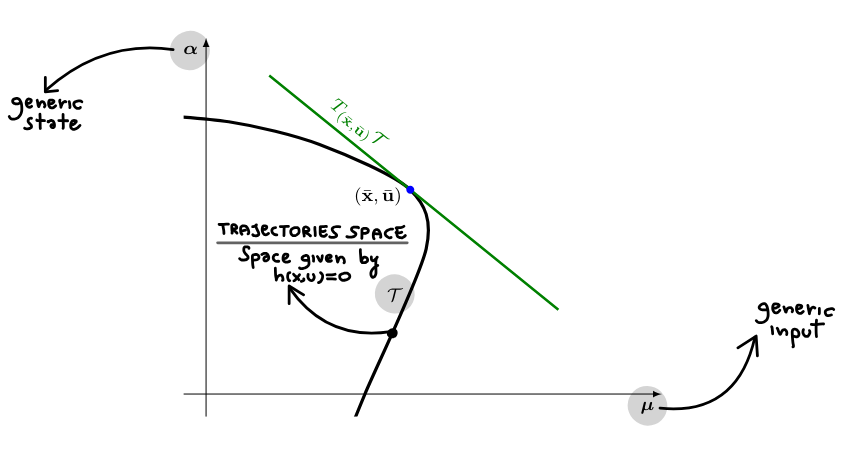
\includegraphics[width=0.7\textwidth]{manifold}
    \caption{Trajectory manifold $\mathcal{T}$}
\end{figure}

Let $\traj\in\mathcal{T}$ be a trajectory of the system, i.e. a point on the trajectory manifold $\mathcal{T}$. The tangent space to $\mathcal{T}$ at a given trajectory (point) $\traj$, denoted as $T_{(\bar{\mathbf{x}},\bar{\mathbf{u}})}\mathcal{T}$, is the set of trajectories satisfying the linearization of $x_{t+1} = f_t(x_t,u_t)$ about the trajectory $(\bar{\mathbf{x}},\bar{\mathbf{u}})$.\\
That is, $T_{(\bar{\mathbf{x}},\bar{\mathbf{u}})}\mathcal{T}=\{(\mathbf{\Delta x, \Delta u})\in\R^{nT}\times\R^{mT}|\nabla_1h(\mathbf{x},\mathbf{u})^T\mathbf{\Delta x} + \nabla_2h(\mathbf{x},\mathbf{u})^T\mathbf{\Delta u} = 0\}$ is the set of trajectories $(\mathbf{\Delta x, \Delta u})$ of
\[
    \Delta x_{t+1} = A_t\Delta x_t + B_t \Delta u_t
\]
with 
\begin{gather*}
    A_t = \nabla_1f_t(\bar{x}_t,\bar{u}_t)^T\\
    B_t = \nabla_2f_t(\bar{x}_t,\bar{u}_t)^T
\end{gather*}

\section{Unconstrained optimal control problem (D-T)}
We look for a solution of the discrete-time optimal control problemm 
\begin{align*}
        \min_{\mathbf{x}\in\R^n,\mathbf{u}\in\R^m} & \displaystyle\sum_{t=0}^{T-1}\ell_t(x_t,u_t)+\ell_T(x_T)\\
        \text{subj. to } & x_{t+1} = f_t(x_t,u_t), \quad t\in\{0,\dots,T-1\} 
\end{align*}
with given initial condition $x_0 = x^0\in \R^n$, where $\ell_t:\R^n\times\R^m\to\R$ and $\ell_T:\R^n\to\R$ are the stage and terminal costs, respectively, and $f_t:\R^n\times\R^m\to\R^n$ are the dynamics of the system.
\begin{remark}
    An optimal control problem constrainded only by the dynamics is called \emph{unconstrained} optimal control problem.
\end{remark}

From now on, we will assume that functions $\ell_t(\cdot,\cdot),\ell_T(\cdot),f_t(\cdot,\cdot)$ are twice continuosly differentiable, i.e. they are class $\mathcal{C}^2$.
Consider the discrete-time system \eqref{system2}. We can introduce the compact notation 
\[
    \mathbf{x} := \begin{bmatrix}
        x_1 \\ \vdots \\ x_T
    \end{bmatrix} \qquad \mathbf{u} := \begin{bmatrix}
        u_0 \\ \vdots \\ u_{T-1}
    \end{bmatrix}
\]
which allows us to write the cost function compactly as 
\[
    \ell({\mathbf{x},\mathbf{u}}) := \sum_{t=0}^{T-1}\ell_t(x_t,u_t)+\ell_T(x_T)
\]
and the equality constraint represented by the dynamics 
\[
    h(\mathbf{x},\mathbf{u}) := \begin{bmatrix}
        f_0(x_0,u_0)-x_1 \\ \vdots \\ f_{T-1}(x_{T-1}u_{T-1})-x_T
    \end{bmatrix}
\]
In light of this compact notation, we can rewrite the optimal control law problem as 
\begin{align*}
    \min_{\mathbf{x}\in\R^{nT},\mathbf{u}\in\R^{mT}} &\ell(\mathbf{x},\mathbf{u})\\
    \text{subj. to } & h(\mathbf{x},\mathbf{u})=0
\end{align*}
where $\ell:\R^{nT}\times\R^{mT}\to\R$ and $h:\R^{nT}\times\R^{mT}\to\R^{nT}$. This is a constrained nonlinear optimization problem with decision variable $(\mathbf{x},\mathbf{u})$.


\section{KKT conditions for unconstrained optimal control}

The Lagrangian function has the form 
\begin{align*}
    \mathcal{L}(\mathbf{x,u,\lambda}) &= \ell(\mathbf{x,u})+\boldsymbol{\lambda}^Th(\mathbf{x,u}) \\
    &= \displaystyle\sum_{t=0}^{T-1}\ell_t(x_t,u_t)+\ell_T(x_T) + \displaystyle\sum_{t=0}^{T-1}\lambda^T_{t+1}(f_t(x_t,u_t)-x_{t+1}) \\
    &= \displaystyle\sum_{t=0}^{T-1}\left(\ell_t(x_t,u_t)+\lambda^T_{t+1}(f_t(x_t,u_t)-x_{t+1})\right)+\ell_T(x_T) \\
    &=\displaystyle\sum_{t=0}^{T}\mathcal{L}_t(x_t,u_t,\boldsymbol{\lambda})
\end{align*}
where $\boldsymbol{\lambda}\in\R^{nT}$ and 
\begin{align*}
    \mathcal{L}_0(x_0,u_0,\boldsymbol{\lambda}) &= \ell_0(x_0,u_0)+\lambda_1^T f_0(x_0,u_0)\\
    \mathcal{L}_t(x_t,u_t,\boldsymbol{\lambda}) &= \ell_t(x_t,u_t)+\lambda_1^T f_t(x_t,u_t)-\lambda_tx_t\\
    \mathcal{L}_T(x_T,\boldsymbol{\lambda}) &= \ell_T(x_T) - \lambda_T^Tx_T
\end{align*}
Let $(\mathbf{x}^*,\mathbf{u}^*)$ be a regular point for the dynamics constraints and an optimal (state-input) trajectory. Then there exists $\boldsymbol{\lambda}^*$ such that $\nabla \mathcal{L}(\mathbf{x}^*,\mathbf{u}^*,\boldsymbol{\lambda}^*)=0$ 

Let us explicitly write condition $\nabla_{(1,2)} \mathcal{L}(\mathbf{x}^*,\mathbf{u}^*,\boldsymbol{\lambda}^*) = 0 $ 
\[
    \nabla_{(1,2)} \mathcal{L}(\mathbf{x}^*,\mathbf{u}^*,\boldsymbol{\lambda}^*) = \begin{bmatrix}
        \nabla_1\mathcal{L}(\mathbf{x}^*,\mathbf{u}^*,\boldsymbol{\lambda}^*)\\
        \nabla_2\mathcal{L}(\mathbf{x}^*,\mathbf{u}^*,\boldsymbol{\lambda}^*)
    \end{bmatrix} = 0
\]
Let us note that 
\[
    \nabla_1\mathcal{L}(\mathbf{x}^*,\mathbf{u}^*,\boldsymbol{\lambda}^*) = \at{\begin{bmatrix}
            \displaystyle\frac{\partial \mathcal{L}(\mathbf{x},\mathbf{u},\boldsymbol{\lambda})}{\partial (x_1)_1}\\
            \vdots \\
            \displaystyle\frac{\partial \mathcal{L}(\mathbf{x},\mathbf{u},\boldsymbol{\lambda})}{\partial (x_1)_n}\\
            \vdots \\
            \displaystyle\frac{\partial \mathcal{L}(\mathbf{x},\mathbf{u},\boldsymbol{\lambda})}{\partial (x_T)_1}\\
            \vdots \\
            \displaystyle\frac{\partial \mathcal{L}(\mathbf{x},\mathbf{u},\boldsymbol{\lambda})}{\partial (x_T)_n}
    \end{bmatrix}}{\mathbf{x}=\mathbf{x}^*}
\]
Since $\mathcal{L}(\mathbf{x},\mathbf{u},\boldsymbol{\lambda})= \displaystyle\sum_{t=0}^{T}\mathcal{L}(x_t,u_t,\boldsymbol{\lambda})$, we can exploit this sparsity and write 
\begin{align*}
    \nabla_2\mathcal{L}_0(x_0,u_0,\boldsymbol{\lambda}) = 0 \qquad & \nabla_2\ell_0(x_0,u_0) + \nabla_2f_0(x_0,u_0)\lambda_1\\
    \begin{bmatrix}
        \nabla_1\mathcal{L}_t(x_t,u_t,\boldsymbol{\lambda})\\
        \nabla_2\mathcal{L}_t(x_t,u_t,\boldsymbol{\lambda})
    \end{bmatrix} = 0 \qquad &  
    \begin{bmatrix}
        \nabla_1\ell_t(x_t,u_t) + \nabla_1f_t(x_t,u_t)\lambda_{t+1}-\lambda_t \\
        \nabla_2\ell_t(x_t,u_t) + \nabla_2f_t(x_t,u_t)\lambda_{t+1}
    \end{bmatrix} = 0 \quad t=1,\dots,T-1 \\
    \nabla_1\mathcal{L}_t(x_t,\boldsymbol{\lambda}) = 0\qquad & \nabla\ell_T(x_T)-\lambda_T = 0
\end{align*}
Let us introduce $A_{t}^{*}$ and $B_{t}^{*}$ that are the state and input matrix of the linearization of the dynamics around the optimal trajectory $(\mathbf{x}^*,\mathbf{u}^*)$:
\begin{gather*} 
    \nabla_1\ell_t(x_t^*,u_t^*) = a_t^*\in \R^n\\
    \nabla_1f_t(x_t^*,u_t^*) = A_{t}^{*T} \quad \text{where } A_t^* = \left.\frac{\partial f_t(x_t,u_t)}{\partial x_t}\right|_{(x_t^*,u_t^*)} \\
    \nabla_2\ell_t(x_t^*,u_t^*) = b_t^*\in \R^n\\
    \nabla_2f_t(x_t^*,u_t^*) = B_{t}^{*T} \quad \text{where } B_t^* = \left.\frac{\partial f_t(x_t,u_t)}{\partial u_t}\right|_{(x_t^*,u_t^*)}
\end{gather*}
So we can rewrite the KKT conditions for unconstrained optimal control as:
\begin{flalign*}
    &a_t^* + A_{t}^{*T}\lambda_{t+1}^* - \lambda_t^* = 0  \qquad t=T-1,\dots,1\\
    &b_t + B_{t}^{*T}\lambda_{t+1}^* = 0 \qquad t=0,\dots,T-1 \\
    &\nabla\ell_T(x_T^*) + \lambda_T^* = 0
\end{flalign*}

These equations form the basis for solving an optimal control problem using the KKT conditions. The process involves defining an iterative algorithm that starts with an initial guess of the input trajectory and then iterates through the following procedure (for a generic step \( k \)) until convergence is achieved.

\subsection{Indirect methods for optimal control}
Given an initial guess for the input trajectory $\mathbf{u}^k = \col(u_0^k,\ldots,u_{T-1}^k)$, the algorithm proceeds as follows:
\begin{enumerate} 
    \item \textbf{Run "forward"} 
        \[
            x_{t+1}^k = f_t(x_t^k,u_t^k), \quad x_0^k = x_{\text{init}}, \quad t=0,\ldots,T-1
        \]
    \item \textbf{Run "backward"}
        \[
            \lambda_t^k = A_{t}^{kT}\lambda_{t+1}^k + a_t^k
        \]
        starting from $\lambda_T^k = \nabla \ell_T (x_T^k)$, to obtain $\lambda_t^k = col(\lambda_1^k,\ldots,\lambda_T^k)$
    \item \textbf{Given $\lambda_t^k$ solve:}
        \[
            b_t + B_{t}^{*T}\lambda_{t+1}^* =\nabla_2\ell(x_t^0,u_t) + \nabla_2f(x_t^0,u_t)\lambda_{t+1}^0 = 0 \quad t=0,\dots,T-1
        \]
        to get $u^{k+1}=\col(u_0^{k+1},\ldots,u_{T-1}^{k+1})$
\end{enumerate}


\section{KKT conditions for constrained optimal control}
We look for a solution of the discrete-time optimal control problem
\begin{align*}
        \min_{x_0\in\R^n,\mathbf{x}\in\R^{nT},\mathbf{u}\in\R^{mT}} & \displaystyle\sum_{t=0}^{T-1}\ell_t(x_t,u_t)+\ell_T(x_T) \\
        \text{subj. to } & x_{t+1} = f_t(x_t,u_t), \quad t=0,\dots,T-1\\
                        & r(x_0,x_T) = 0 \\
                        & g_t(x_t,u_t)\leq 0 ,\quad t=0,\dots,T-1
\end{align*}
where 
\begin{itemize}
    \item $\ell_t:\R^n\times\R^m\to\R$ is the stage cost,
    \item $\ell_T:\R^n\to\R$ is the terminal cost,
    \item $r: \R^n\times\R^n\to\R^{p_0}$ identifies a \emph{boundary constraint} on initial and final states,
    \item $g_t:\R^n\times\R^m\to\R^p$ for each $t$ identifies \emph{point-wise constraints} on state and input at some time $t$
\end{itemize}
The Lagrangian function has the form 
\begin{align*}
    \mathcal{L}(\mathbf{x},\mathbf{u},\boldsymbol{\lambda},\boldsymbol{\mu}) =& \ell(\mathbf{x},\mathbf{u})+\boldsymbol{\lambda}_d^T h(\mathbf{x},\mathbf{u})+ \lambda_b^T r(x_0,x_T) + \boldsymbol{\mu}^Tg(\mathbf{x},\mathbf{u}) \\ 
    =&\displaystyle\sum_{t=0}^{T-1}\ell_t(x_t,u_t)+\ell_T(x_T) + \displaystyle\sum_{t=0}^{T-1}\lambda_{d,t+1}(f_t(x_t,u_t)-x_{t+1})+\lambda_b^Tr(x_0,x_T) + \displaystyle\sum_{t=0}^{T-1}\mu_t^Tg_t(x_t,u_t)\\
    =&\displaystyle\sum_{t=0}^{T}\mathcal{L}_t(x_t,u_t,\boldsymbol{\lambda},\boldsymbol{\mu})
\end{align*}
where
\begin{align*}
    \mathcal{L}_0(x_0,u_0,\boldsymbol{\lambda},\boldsymbol{\mu}) &= \ell_0(x_0,u_0)+\lambda_{d,1}^T f_0(x_0,u_0) + \lambda_{b,0}r_0(x_0)\\
    \mathcal{L}_t(x_t,u_t,\boldsymbol{\lambda}) &= \ell_t(x_t,u_t)+\lambda_1^T f_t(x_t,u_t)-\lambda_tx_t+\mu_t^Tg_t(x_t,u_t) \qquad t=1,\dots,T-1\\
    \mathcal{L}_T(x_T,\boldsymbol{\lambda}) &= \ell_T(x_T) - \lambda_T^Tx_T + \lambda_{b,T}^Tr_T(x_T)
\end{align*}
and we assumed $r(x_0,x_T)=\col(r_0(x_0),r_T(x_T))$ and $\lambda_b = \col(\lambda_{b,0},\lambda_{b,T})$.

Let $(\mathbf{x}^*,\mathbf{u}^*)$ be a regular point for the dynamics constraints and an optimal (state-input) trajectory. 
Then there exists $\boldsymbol{\lambda}^*$ and $\boldsymbol{\mu}^*>0$ such that $\nabla \mathcal{L}(\mathbf{x}^*,\mathbf{u}^*,\boldsymbol{\lambda}^*)=0$ + complementary slackness conditions.

Let us explicitly write condition $\nabla_{(1,2)} \mathcal{L}(\mathbf{x}^*,\mathbf{u}^*,\boldsymbol{\lambda}^*,\boldsymbol{\mu}^*) = 0 $ 
\[
    \nabla_{(1,2)} \mathcal{L}(\mathbf{x}^*,\mathbf{u}^*,\boldsymbol{\lambda}^*,\boldsymbol{\mu}^*) = \begin{bmatrix}
        \nabla_1\mathcal{L}(\mathbf{x}^*,\mathbf{u}^*,\boldsymbol{\lambda}^*,\boldsymbol{\mu}^*)\\
        \nabla_2\mathcal{L}(\mathbf{x}^*,\mathbf{u}^*,\boldsymbol{\lambda}^*,\boldsymbol{\mu}^*)
    \end{bmatrix} = 0
\]
Since $\mathcal{L}(\mathbf{x},\mathbf{u},\boldsymbol{\lambda}^*,\boldsymbol{\mu}^*)= \displaystyle\sum_{t=0}^{T}\mathcal{L}(x_t,u_t,\boldsymbol{\lambda})$, we can exploit this sparsity and write 
\begin{align*}
    \begin{bmatrix}
        \nabla_1\mathcal{L}_0(x_0,u_0,\boldsymbol{\lambda},\boldsymbol{\mu}) \\
        \nabla_2\mathcal{L}_0(x_0,u_0,\boldsymbol{\lambda},\boldsymbol{\mu}) 
    \end{bmatrix} = 0 \qquad &
    \begin{bmatrix}
        \nabla_1\ell(x_0,u_0)\nabla_1f_0(x_0,u_0)\lambda_1+\nabla r_0(x_0)\lambda_{b,0}+\nabla_1g_t(x_0,\mu_0)\\
        \nabla_2\ell_0(x_0,u_0)\nabla_2f_0(x_0,u_0)\lambda_1 + \nabla_2g_t(x_0,u_0)\mu_0\\
    \end{bmatrix} = 0\\
    \begin{bmatrix}
        \nabla_1\mathcal{L}_t(x_t,u_t,\boldsymbol{\lambda})\\
        \nabla_2\mathcal{L}_t(x_t,u_t,\boldsymbol{\lambda})
    \end{bmatrix} = 0 \qquad &  
    \begin{bmatrix}
        \nabla_1\ell_t(x_t,u_t) + \nabla_1f_t(x_t,u_t)\lambda_{t+1}-\lambda_t + \nabla_1g_t(x_t,u_t)\mu_t\\
        \nabla_2\ell_t(x_t,u_t) + \nabla_2f_t(x_t,u_t)\lambda_{t+1} + \nabla_2g_t(x_t,u_t)\mu_t
    \end{bmatrix} = 0 \quad t=1,\dots,T-1 \\
    \nabla_1\mathcal{L}_t(x_t,\boldsymbol{\lambda}) = 0\qquad & \nabla\ell_T(x_T)-\lambda_T + \nabla r_T(x_T)\lambda_{b,T} = 0
\end{align*}
for $(x_t,u_t,\lambda_t,\mu_t) = (x_t^*,u_t^*,\lambda_t^*,\mu_t^*)$


\chapter{Linear Quadratic (LQ) Optimal Control}

Consider a linear quadratic optimal control problem as: 
\begin{align*}
        \min_{\substack{x_1,\dots,x_T \\ u_0,\dots,u_{T-1}}} & \displaystyle\sum_{t=0}^{T-1}\displaystyle\frac{1}{2}[x_t^TQ_tx_t+u_t^TR_tu_t] + \displaystyle\frac{1}{2}x_T^TQ_Tx_T\\
        \text{subj. to } & x_{t+1} = A_tx_t + B_tu_t \quad t=0,\dots,T-1\\
                        &x_0 = x_{\text{init}}
\end{align*}
We assume $Q_t=Q_t^T\geq 0,\ $ for $ t=0,\dots,T-1$, $Q_T = Q_T^T \geq 0$, and $R_t=R_t^T > 0 \ $ for $t=0,\dots,T-1$

\section{First order optimality condition}

\textbf{Recall} the first order necessary and sufficient conditions for $(\mathbf{x}^*,\mathbf{u}^*)$ to be an optimal trajectory $\exists \boldsymbol{\lambda}^*$ such that:
\begin{align*}
    x^*_{t+1} &= f_t(x^*_t, u^*_t) & t &= 0,\ldots,T-1 \\
    \lambda^*_t &= \nabla_1 f_t(x^*_t, u^*_t)\lambda^*_{t+1} + \nabla_1 \ell_t(x^*_t, u^*_t) & t &= T-1,\ldots,1 \\
    0 &= \nabla_2 f_t(x^*_t, u^*_t)\lambda^*_{t+1} + \nabla_2 \ell_t(x^*_t, u^*_t) & t &= 0,\ldots,T-1
\end{align*}
$\text{with } x^*_0 = x_{\text{init}} \text{ and } \lambda^*_T = \nabla\ell_T(x^*_T).$\\
In the case of the LQ problem becomes:
\begin{gather*}
    \nabla_1f_t(x_t,u_t) = A_t^T\\
    \nabla_1\ell(x_t,u_t) = \nabla_1(\displaystyle\frac{1}{2}x_t^TQ_tx_t+\displaystyle\frac{1}{2}u_t^TR_tu_t)=Q_tx_t\\
    \nabla_2f_t(x_t,u_t) = B_t^T\\
    \nabla_2\ell_t(x_t,u_t) = R_tu_t\\
\end{gather*}
Therefore :
\begin{gather*}
    x^*_{t+1} = A_tx^*_t + B_tu^*_t \quad t=0,\dots,T-1\\
    \lambda_t^* = A_t^T\lambda_{t+1}^* + Q_tx_t^* \quad t=T-1,\dots,0\\
    0 = B_t^T\lambda_{t+1}^* + R_tu_t^* \quad t=0,\dots,T-1
\end{gather*}
$\text{with } x^*_0 = x_{\text{init}} \text{ and } \lambda^*_T = Q_Tx^*_T.$

\begin{remark}
second order optimality conditions 
\[
    y^T\nabla^2_{(1,2)(1,2)}\mathcal{L}(\mathbf{x}^*,\mathbf{u}^*,\boldsymbol{\lambda}^*,)y \geq 0
\]

%%%%%%%%%%%%%%%%%%%%%%%%%%%%%%%%%%%%%%%%%%%%%%%%%%%%%%%%%%%%%%%%%%%%%%%%%%%%%%%%%%%%%%%%%%%%%%%%%%%%%%%%%%%%%%%%%%%%%%%%%%%%%%%%%%%%%%%%%%%%%%%%%%%%%%%%%%%%%%%%%%%%%%%%%%%%%%
\section{LQ problem: Optimal solution}
For vectors $y$ satisfying the "linear approximation of the constraint". The hessian turns out as 
\[
    \begin{bmatrix}
        Q_1 & & &  0\\
            & \ddots & & & \\ 
        0 & & & Q_n
    \end{bmatrix}
\]
\end{remark}
Because $R_t>0$ it is invertible, we can write 
\[
    u_t^* = -R_t^{-1}B_t^T\lambda_{t+1}^*
\]
Introducing a matrix $P_t=P_t^T \geq 0$, it can be proven that 
\[
    \lambda_t^* = P_tx_t^*
\]
Assuming that it holds for some $t\leq T-1$, then we have 
\[
    u_t^* = -R_t^{-1}B_t^TP_{t+1}x_{t+1}^*
\]
Now, considering the constraint represented by the dynamics 
\[
    u_t^* = -R_t^{-1}B_t^TP_{t+1}(A_tx_t^*+B_tu_t^*)
\]
Solving by $u^*_t$ yields 
\[
    u_t^* = -(R_t+B_t^Tp_{t+1}B_t)^{-1}B_t^TP_{t+1}A_tx^*_t \quad t=0,\dots,T-1
\]
we get 
\begin{gather*}
    u_t^* = -R_t^{-1}B_t^Tp_{t+1}x_{t+1}^* \\
    = -R_t^{-1}B_t^TP_{t+1}(A_tx_t^*+B_tu_t^*)
\end{gather*}
we multiply both sides by $R_t$: 
\begin{gather*}
    R_tu_t^* = -B_t^TP_{t+1}(A_tx_t^*+B_tu_t^*)\\
    R_tu_t^* = -B_t^TP_{t+1}A_tx_t^*-B_t^TP_{t+1}B_tu_t^*\\
    (R_t+B_t^TP_{t+1}B_t)u_t^* = -B_t^TP_{t+1}A_tx_t^*
\end{gather*}
The matrix on the left is clearly positive definite, therefore: 
\[
    u_t^* = -(R_t+B_t^TP_{t+1}B_t)^{-1}B_t^TP_{t+1}A_tx_t^*
\]
which we can write as 
\[
    u_t^* = K_t^*x_t^*
\]
that is, the optimal control is a state feedback with gain $-(R_t+B_t^TP_{t+1}B_t)^{-1}B_t^TP_{t+1}$
\[
    x_{t+1}^* = A_tx_t^*-B_t(R_t+B_t^TP_{t+1}B_t)^{-1}B_t^TP_{t+1}A_tx_t^*
\]
which we can rewrite as 
\[
    x_{t+1}^* = (A_t-B_t(R_t+B_t^TP_{t+1}B_t)^{-1}B_t^TP_{t+1}A_t)x_t^*
\]
which is a closed loop system. We multiply both sides by $P_{t+1}$ and obtain 
\[
    P_{t+1}x_{t+1}^* = P_{t+1}(A_t-B_t(R_t+B_t^TP_{t+1}B_t)^{-1}B_t^TP_{t+1}A_t)x_t^*
\]
On the left side of the equation we have obtained $\lambda_{t+1}^*$
\[
    \lambda_{t+1}^* =P_{t+1}(A_t-B_t(R_t+B_t^TP_{t+1}B_t)^{-1}B_t^TP_{t+1}A_t)x_t^*
\]
Remembering that $\lambda_t^* = A_t^T\lambda_{t+1}^*+Q_tx_t^*$ we multiply both sides by $A_t^T$ and then add $Q_tx^*_t$ and obtain 
\[
    A_t^T\lambda_{t+1}^*+Q_tx_t^*=A_t^TP_{t+1}(A_t-B_t(R_t+B_t^TP_{t+1}B_t)^{-1}B_t^TP_{t+1}A_t)x_t^* + Q_tx_t^*
\]
and because 
\[
    \lambda_t^* = P_tx_t^*
\]
then 
\[
    P_tx_t^* = [A_t^TP_{t+1}(A_t-B_t(R_t+B_t^TP_{t+1}B_t)^{-1}B_t^TP_{t+1}A_t)+Q_t]x_t^*
\]
so 
\[
    P_tx_t^* = \left[A_t^TP_{t+1}A_t-A_t^TP_{t+1}B_t(R_t+B_t^TP_{t+1}B_t)^{-1}B_t^TP_{t+1}A_t+Q_t\right]x_t^*
\]
from which 
\begin{equation}\label{Riccati}
    P_t = A_t^TP_{t+1}A_t-A_t^TP_{t+1}B_t(R_t+B_t^TP_{t+1}B_t)^{-1}B_t^TP_{t+1}A_t+Q_t
\end{equation}
because $\lambda_T^*=Q_Tx_T^*$ we have that 
\[
    P_T = Q_T
\]
Therefore, by propagating equation \eqref{Riccati} back in time, $P_t$ can be calculated. Equation \eqref{Riccati} is called difference Riccati equation
\begin{itemize}
    \item gains $K_t^*$ can be precomputed offline and then used for different $x_0$ 
    \item It can be shown that if $T\to\infty$ the gains $K_t^*$ converge and asymptotically stabilize the system
\end{itemize}
\subsubsection{Other formulations of the Riccati equation}
The usual Riccati recursion reads:
\[
    P_t = Q_t + A_t^TP_{t+1}A_t - A_t^TP_{t+1}B_t(R_t+B_t^TP_{t+1}B_t)^{-1}B_t^TP_{t+1}A_t
\]
by exploiting the matrix inversion lemma\footnote{$(A+BC)^{-1} = A^{-1}-A^{-1}B(I+CA^{-1}B)^{-1}CA^{-1}$}, we can write: 
\begin{align*}
    P_t &= Q_t + A_t^TP_{t+1}A_t - A_t^TP_{t+1}B_t(R_t+B_t^TP_{t+1}B_t)^{-1}B_t^TP_{t+1}A_t\\
    P_t &= Q_t + A_t^TP_{t+1}(I-B_t(R_t+B_t^TP_{t+1}B_t)^{-1}B_t^TP_{t+1})A_t\\
    P_t &= Q_t + A_t^TP_{t+1}(I-B_t((I+B_t^TP_{t+1}B_tR_t^{-1})R_t)^{-1}B_t^TP_{t+1})A_t\\
    P_t &= Q_t + A_t^TP_{t+1}(I-B_tR_t^{-1}(I+B_t^TP_{t+1}B_tR_t^{-1})^{-1}B_t^TP_{t+1})A_t\\
    P_t &= Q_t + A_t^TP_{t+1}(I-B_tR_t^{-1}B_t^TP_{t+1})A_t\\
    P_t &= Q_t + A_t^T(I-B_tR_t^{-1}B_t^TP_{t+1})P_{t+1}A_t
\end{align*}
\section{Infinite horizion LQ optimal control}
Consider the infinite-horizon optimal control problem
\begin{align*}
        \min_{\substack{x_1,x_2,\dots \\ u_0,u_1,\dots}} & \displaystyle\sum_{t=0}^{\infty}\displaystyle\frac{1}{2}\left[x_t^TQx_t+u_t^TRu_t\right] \\
        \text{subj. to } & x_{t+1} = Ax_t + Bu_t \quad t=0,1,\dots\\
                        &x_0 = x_{\text{init}}
\end{align*}
where 
\begin{itemize}
    \item $x\in\R^n$ and $u\in\R^m$
    \item $A\in\R^{n\times n}$
    \item $B\in\R^{n\times m}$
    \item $Q\in\R^{n\times n}$ and $Q=Q^T\geq 0$
    \item $R\in\R^{m\times m}$ and $R=R^T> 0$
\end{itemize}
We assume the pair $(A,B)$ is controllable and the pair $(A,C)$ with $Q=C^TC$ is observable
Let us write 
\[
    y_t=Cx_t
\]
which leads to 
\[
    \displaystyle\frac{1}{2}x_t^TQx_t = \displaystyle\frac{1}{2}x_t^TC^TCx_t = \displaystyle\frac{1}{2}y_t^Ty_t
\]
The controllability assumption guardantees that an optimal controller exists: if $(A,B)$ controllable, then $\exists \bar{u}_0,\dots,\bar{u}_{T-1}$ for $T$ sufficiently large ($T=n$) such that $\forall x_0\in \R^n\implies x_T=0$. Consider the input
\[
    \bar{u}_0,\dots,\bar{u}_{T-1},0,\dots,0,\dots
\]
Let us compute the cost associated to this input 
\[
    \displaystyle\sum_{t=0}^{\infty}\displaystyle\frac{1}{2}[x_t^TQx_t+u_t^TRu_t] =\displaystyle\sum_{t=0}^{T-1}\displaystyle\frac{1}{2}\bar{x}_t^TQ\bar{x}_t + \displaystyle\frac{1}{2}\bar{u}_t^TR\bar{u}_t
\]
We can note that the cost is a finite quantity. Because the cost is finite, There must exist a solution which minimizes the cost.
\proposition

Let the pair $(A,B)$ be controllable and the pair $(A,C)$ with $Q=C^TC$ be observable. Then the following holds:
\begin{itemize}
    \item there exists a unique positive definite $P_\infty$ equilibrium solution of the Difference Riccati Equation. That is, $P_\infty$ is a solution of \[
            P_\infty = Q+A^TP_\infty A-A^TP\infty B(R+B^TP_\infty B)^{-1}B^TP_\infty A
        \]
        which is called \emph{Algebraic Riccati Equation }
        \item the optimal control is a feedback of the state given by:
            \begin{flalign*}
                & K^* = -(R+B^TP_\infty B)^{-1}(B^TP_\infty A)\\
                & u_t^* = K^*x^*_t\\
                & x_{t+1}^* = Ax_t^*+Bu_t^* \quad t=1,2,\dots \quad x_0^* = X_{\text{init}}
            \end{flalign*}
\end{itemize}
\remark The observability of $(A,C)$ guardantees that if the stage cost goes to zero, then the state trajectory goes to zero.

\section{Affine LQR}
Consider a LQR problem with affine cost and affine dynamics 
\begin{align*}
    \min_{\substack{x_1,\dots,x_T\\u_0,\dots,u_{T-1}}} & \displaystyle\sum_{t=0}^{T-1} \begin{bmatrix}
        q_t \\ r_t
    \end{bmatrix}^T \begin{bmatrix}
        x_t \\ u_t
    \end{bmatrix}  + \begin{bmatrix}
        x_t \\ u_t
    \end{bmatrix}^T \begin{bmatrix}
        Q_t & S_t^T \\ S_t & R_t
    \end{bmatrix} \begin{bmatrix}
        x_t \\ u_t
    \end{bmatrix} + q_t^Tx_T + x_T^TQ_Tx_T\\ 
    \text{subj. to } & x_{t+1} = A_tx_t + B_tu_t + c_t \quad t = 0,\dots,T-1 
\end{align*}
where $Q_t=Q_t^T\geq 0$, $R_t=R_t^T>0$, $S_t$ such that the problem is convex, i.e. $Q_t-S_t^TR_t^{-1}S_t\geq 0$

This problem can be conveniently solved by augmenting the state as 
\[
    \tilde{x}_t := \begin{bmatrix}
        1 \\ x_t
    \end{bmatrix}
\]
we can rewrite the cost and system matrices as 
\[
    \tilde{Q}_t := \begin{bmatrix}
        0 & q_t^T \\ q_t  & Q_t
    \end{bmatrix} \quad \tilde{S}_t := \begin{bmatrix}
        r_t & S_t
    \end{bmatrix} \quad \tilde{R}_t := R_t \quad \tilde{A}_t := \begin{bmatrix}
        1 & 0 \\ c_t & A_t
    \end{bmatrix} \quad \tilde{B}_t := \begin{bmatrix}
        0 \\ B_t
    \end{bmatrix}
\]
Then, we solve the associated LQR problem 
\begin{align*}
    \min_{\substack{x_1,\dots,x_T\\u_0,\dots,u_{T-1}}} & \displaystyle\sum_{t=0}^{T-1}  \begin{bmatrix}
        \tilde{x}_t \\ u_t
    \end{bmatrix}^T \begin{bmatrix}
        \tilde{Q}_t & \tilde{S}_t^T \\ \tilde{S}_t & \tilde{R}_t
    \end{bmatrix} \begin{bmatrix}
        \tilde{x}_t \\ u_t
    \end{bmatrix} + \tilde{x}_T^TQ_T\tilde{x}_T\\ 
    \text{subj. to } & \tilde{x}_{t+1} = \tilde{A}_t\tilde{x}_t + \tilde{B}_tu_t  \quad t = 0,\dots,T-1 \\
    & x_0 = x_{\text{init}}
\end{align*}
The optimal solution of the problem reads 
\begin{align*}
    u_t^* &= K_t^*x_t^* + \sigma_t^*\\ 
    x_{t+1}^* &= A_tx_t^* + B_tu_t^*
\end{align*}
where 
\begin{align*}
    K_t^* &= -(R_t+B_t^TP_{t+1}B_t)^{-1}(S_t+B_t^TP_{t+1}A_t)\\ 
    \sigma_t^* &= -(R_t+B_t^TP_{t+1}B_t)^{-1}(r_t+B_t^Tp_{t+1}+B_t^TP_{t+1}c_t)\\
\end{align*}
\begin{align*}
    p_t &= q_t + A_t^TP_{t+1} + A_t^TP_{t+1}C_t + {K_t^*}^T(R_t+B_t^TP_{t+1}B_t)\sigma_t^*\\
    P_T &= Q_t + A_t^TP_{t+1}A_t - {K_t^*}^*T(R_t+B_t^TP_{t+1}B_t)K_t^*
\end{align*}
with $P_T = Q_T$ and $p_T = q_T$



\chapter{Optimality Conditions for Unconstrained Optimal Control via Shooting}

Let us consider the system dynamics 
\[
    x_{t+1} = f_t(x_t,u_t) \quad t=0,\dots,T-1 \quad x_0 \text{ given}
\]
and let us suppose we have an input sequence $u_0,\dots,u_{T-1}$. We have: 
\begin{flalign*}
    & x_1 =f_0(x_0,u_0) = \tilde{\Phi}_1(\mathbf{u}) \\
    &  x_2 = f_1(x_1,u_1) = f_1(f_0(x_0,u_0),u_1) = \tilde{\Phi}_2(\mathbf{u}) \\
    & \vdots \\
    & x_t = \tilde{\Phi}_t(\mathbf{u}) \qquad t=0,\dots,T-1
    & \vdots \\
    & x_T = \tilde{\Phi}_{T}(\mathbf{u}) \qquad t=0,\dots,T-1
\end{flalign*}
Idea: express the state $x_t$ at each $t=1,\dots,T$ as a function of the input sequence $\mathbf{u}$ unly. For all $t$ we can introduce a map $\Phi_t:\R^m \to \R^n$ such that 
\[
    x_t := \Phi_t(\mathbf{u})
\]
compact notation
\[
    \Phi(\mathbf{u}) = \col(\Phi_1(\mathbf{u}),\dots,\Phi_T(\mathbf{u}))
\]
so that 
\[
    \mathbf{x} = \Phi(\mathbf{u})
\]
Note: Given any arbitrary $\bar{u}_0,\dots,\bar{u}_{T-1}$, we have that $\Phi_{t+1}(\bar{\mathbf{u}}) = f_t(\Phi_t(\bar{\mathbf{u}}),u_t)$ by construction. This is equivalent to the equality constraint for the optimal control problem.

\section{Reduced optimal control problem}\label{shoot}
We can rewrite the optimal control problem as 
\[
    \min_{\mathbf{u}\in\R^{mT}} \displaystyle\sum_{t=0}^{T-1}\ell_t(\Phi_t(\mathbf{u}),u_t)+\ell_T(\Phi_T(\mathbf{u}))
\]
as noted before, the equality constraint is satisfied by construction, making this an unconstrained optimization problem. We can rewrite it compactly as 
\[
    \min_{\mathbf{u}\in\R^{mT}}\ell(\Phi(\mathbf{u}),\mathbf{u})
\]
and by defining $J(\mathbf{u}):=\ell(\Phi(\mathbf{u}),\mathbf{u})$
\[
    \min_{\mathbf{u}\in\R^{mT}} J(\mathbf{u}):
\]
This goes by the name of \emph{reduced} or \emph{condensed optimal control problem}. The procedure of writing $\mathbf{x}$ as a function of $\mathbf{u}$ and then plugging it into the optimal control problem is called shooting.
\begin{remark}
    if we consider path input constraints 
    \begin{align*}
        g_0(u_0)\leq 0 \\
        \vdots \\
        g_{T-1}(u_{T-1})\leq 0 
    \end{align*}
    the problem becomes 
    \begin{align*}
        \min_{\mathbf{u}\in\R^{mT}} & J(\mathbf{u}) \\
        \text{subj to } & g_0(u_0)\leq 0 \\
        & \vdots \\
        & g_{T-1}(u_{T-1})\leq 0 
    \end{align*}
\end{remark}
\begin{remark}
     if we have constraints of the type 
     \begin{align*}
         &g_0(x_0,u_0)\leq 0\\
         &\vdots \\
         &g_{T-1}(x_{T-1},u_{T-1})\leq 0\\
     \end{align*}
     They can be rewritten as functions of $x_0$ and $\mathbf{u}$ only, however $\Phi(\cdot)$ must be explicitly known
\end{remark}

\section{Algorithms for optimal control problem solution}
We can apply the gradient method, i.e. 
\[
    \mathbf{u}^{k+1}=\mathbf{u}^k-\gamma\nabla J(\mathbf{u}^k)
\]
We can formally write the expression of $\nabla J(\mathbf{u})=\nabla \ell(\Phi(\mathbf{u}),\mathbf{u})$ by using the chain rule of differentiation. 
Consider\[
    J(\mathbf{u}) = \ell(\phi(\mathbf{u}),\mathbf{u})
\]
Suppose $\mathbf{u}\in\R$, we have: 
\[
    \displaystyle\frac{d}{d\mathbf{u}}J(\bar{\mathbf{u}}) = \at{\displaystyle\frac{\partial\ell(\mathbf{x},\mathbf{u})}{\partial\mathbf{x}}}{\substack{\mathbf{x} = \phi(\bar{\mathbf{u}})\\ \mathbf{u} = \bar{\mathbf{u}}}}\at{\displaystyle\frac{\partial\phi(\mathbf{u})}{\partial\mathbf{u}}}{\mathbf{u} = \bar{\mathbf{u}}} + \at{\displaystyle\frac{\partial\ell(\mathbf{x},\mathbf{u})}{\partial\mathbf{u}}}{\substack{\mathbf{x} = \phi(\bar{\mathbf{u}})\\ \mathbf{u} = \bar{\mathbf{u}}}}
\]
In general, we have $\mathbf{u}\in\R^{mT}$, Therefore
\[
    \nabla J(\mathbf{u}) = \nabla\phi(\mathbf{u})\nabla_1\ell(\phi(\mathbf{u}),\mathbf{u})+\nabla_2\ell(\phi(\mathbf{u}),\mathbf{u})
\]
However, notice that the calculation of $\nabla J(\mathbf{u})$ requires $\nabla\phi(\mathbf{u})$, which may be difficult to compute.
\[
    \nabla\Phi(\mathbf{u}) = \nabla \begin{bmatrix}
        \Phi_{1,1}(\mathbf{u})\\
        \Phi_{1,2}(\mathbf{u})\\
        \vdots \\
        \Phi_{t,1}(\mathbf{u})\\
        \Phi_{t,2}(\mathbf{u})\\
        \vdots
    \end{bmatrix}
\]
\[
    \nabla\Phi(\mathbf{u}) = \begin{bmatrix}
        \displaystyle\frac{\partial \Phi_{1,1}}{\partial u_0} & \displaystyle\frac{\partial \Phi_{1,2}}{\partial u_0} & \cdots & \displaystyle\frac{\partial \Phi_{T,n}}{\partial u_0}\\
        \vdots & \vdots & \ddots & \vdots \\
        \displaystyle\frac{\partial \Phi_{1,1}}{\partial u_{T-1}} & \displaystyle\frac{\partial \Phi_{1,2}}{\partial u_{T-1}} &\cdots & \displaystyle\frac{\partial \Phi_{T,n}}{\partial u_{T-1}}
    \end{bmatrix}
\]
where $\Phi_{t,j}:\R^{mT}\to \R$, therefore the above matrix is a matrix of scalars.
Let us introduce an auxiliary function $\mathcal{L}(\mathbf{x},\mathbf{u},\boldsymbol{\lambda}):\R^{nT}\times \R^{mT} \times\R^{nT}\to \R$ given by 
\[
    \mathcal{L}(\mathbf{x},\mathbf{u},\boldsymbol{\lambda})=\ell(\mathbf{x},\mathbf{u})+h(\mathbf{x},\mathbf{u})^T\boldsymbol{\lambda}
\]
where $\boldsymbol{\lambda}\in\R^{nT}$ is a "costate vector" and 
\[
    h(\mathbf{x},\mathbf{u}) = \begin{bmatrix}
         f_0(x_0,u_0)-x1\\
         \vdots \\
         f_{T-1}(x_{T-1}u_{T-1})-x_T
    \end{bmatrix}
\]
To compute $\nabla J(\mathbf{u})$ let us evaluate $\mathcal{L}(\cdot)$ for $\mathbf{x} = \Phi(\mathbf{u})$. Since $h(\Phi(\mathbf{u},)\mathbf{u})=0$ it holds that 
\[
    \mathcal{L}(\Phi(\mathbf{u}),\mathbf{u},\boldsymbol{\lambda}) = J(\mathbf{u}) \quad \forall \lambda\in\R^{nT}
\]
Therefore 
\[
    \nabla \mathcal{L}(\Phi(\mathbf{u}),\mathbf{u},\boldsymbol{\lambda}) = \nabla J(\mathbf{u}) \quad \forall \boldsymbol{\lambda}
\]
hence we can write 
\[
    \nabla J (\mathbf{u}) = \nabla\Phi(\mathbf{u})(\nabla_1\ell(\Phi(\mathbf{u}),\mathbf{u})+\nabla_1 h(\Phi(\mathbf{u}),\mathbf{u})\boldsymbol{\lambda})+\nabla_2\ell(\Phi(\mathbf{u}),\mathbf{u})+\nabla_2 h(\Phi(\mathbf{u}),\mathbf{u})\boldsymbol{\lambda}
\]
which holds for every $\boldsymbol{\lambda}$. Therefore, for a given $\mathbf{u}$, we can cleverly select $\boldsymbol{\lambda}=\boldsymbol{\lambda}(\mathbf{u})$ such that: 
\[
    \nabla_1\ell(\Phi(\mathbf{u}),\mathbf{u})+\nabla_1h(\Phi(\mathbf{u}),\mathbf{u})\boldsymbol{\lambda}(\mathbf{u}) = 0
\]
which leads to 
\[
    \nabla J(\mathbf{u}) = \nabla_2\ell(\phi(\mathbf{u}),\mathbf{u})+\nabla_2 h(\phi(\mathbf{u}),\mathbf{u})\boldsymbol{\lambda}(\mathbf{u})
\]
By recalling that 
\[
    \mathcal{L}(\mathbf{x},\mathbf{u},\boldsymbol{\lambda}) = \ell(\mathbf{x},\mathbf{u})+\boldsymbol{\lambda}^Th(\mathbf{x},\mathbf{u})
\]
We have
\[
    \nabla J(\mathbf{u}) = \nabla\phi(\mathbf{u})\nabla_1\mathcal{L}(\Phi(\mathbf{u}),\mathbf{u},\boldsymbol{\lambda})+\nabla_2\mathcal{L}(\Phi(\mathbf{u}),\mathbf{u},\boldsymbol{\lambda})
\]
so that choosing $\boldsymbol{\lambda} = \boldsymbol{\lambda}(\mathbf{u})$ such that
\[
    \nabla_1\mathcal{L}(\Phi(\mathbf{u}),\mathbf{u},\boldsymbol{\lambda}(\mathbf{u})) = 0
\]
it holds 
\[
    \nabla J(\mathbf{u}) = \nabla_2\mathcal{L}(\Phi(\mathbf{u}),\mathbf{u},\boldsymbol{\lambda}(\mathbf{u}))
\]




\subsection{First order necessary condition for optimality}
Let $\mathbf{u}^*$ be a local minimum with $\mathbf{x}^* = \Phi(\mathbf{u}^*)$ 
Then
\[
    \nabla J(\mathbf{u^*}) = 0
\]
that is, if there exists a $\boldsymbol{\lambda}^*$ such that 
\[
    \nabla_1\mathcal{L}(\Phi(\mathbf{u}^*),\mathbf{u}^*,\boldsymbol{\lambda}^*)=0
\]
it holds 
\[
    \nabla_2\mathcal{L}(\Phi(\mathbf{u}^*),\mathbf{u}^*,\boldsymbol{\lambda}^*)=0
\]
\subsection[Explicit computation of the gradient of the shooting cost function]{Explicit computation of $\nabla J(\mathbf{u})$}
\[
    \mathcal{L}(\mathbf{x},\mathbf{u},\boldsymbol{\lambda}) = \displaystyle\sum_{t=0}^{T-1}[\ell_t(x_t,u_t)+\lambda_{t+1}^T f_t(x_t,u_t)-\lambda_{t+1}x_{t+1}]+\ell_T(x_T)% = \displaystyle\sum_{t=0}^{T-1}(x_t,u_t)
\]
By writing out the sum we can easily calculate $\nabla_1\mathcal{L}(\phi(\mathbf{u},\mathbf{u},\mathbf{x}))=0$ for each $x_t$: 
\begin{gather*}
    \mathcal{L}(\mathbf{x},\mathbf{u},\boldsymbol{\lambda})= \ell_0(x_0,u_0)+ \lambda_1^Tf_0(x_0,u_0)-\lambda_1x_1+ \ell_1(x_1,u_1)+\lambda_2^Tf_1(x_1,u_1)-\lambda_2x_2+\dots\\
    \nabla_t\ell_t(x_t,u_t)+\nabla_t f_t(x_t,u_t)\lambda_{t+1}- \lambda_t = 0\\
    \nabla\ell_T(x_T) - \lambda_T = 0
\end{gather*}
which leads to 
\begin{align*}
    \lambda_T &= \nabla\ell_T(x_T)\\
    \lambda_t &= \nabla_t\ell_t(x_t,u_t)+\nabla_t f_t(x_t,u_t)\lambda_{t+1}  \quad t = T-1,\dots,1
\end{align*}
then
\[
    (\nabla J(u))_t = \nabla_2\ell_t(x_t,u_t)+\nabla_2f_t(x_t,u_t)\lambda_{t+1} 
\]
Notice we can write 
\begin{flalign*}
    & A_t^T = \nabla_1f(x_t,u_t)\\
    & B_t^T = \nabla_2f(x_t,u_t) 
\end{flalign*}  
so that we can rewrite
\begin{align*}
    \lambda_t &= A_t^T\lambda_t+1 + a_t\\
    (\nabla J(u))_t &= B_t^T\lambda_{t+1}+b_t
\end{align*}
so given $u_0,\dots,u_{T-1}$ and $x_1,\dots,x_T$ such that $x_{t+1}=f(x_t,u_t)$ we can compute $\lambda_T,\dots,\lambda_1$ running backwards. 
\begin{remark}
    $A_t\in\R^{n\times n}$ and $B_t\in\R^{n\times m}$ are the state and input matrices of the linearization of the system $x_{t+1} = f(x_t,u_t)$ about the trajectory $(\mathbf{x},\mathbf{u})$
\end{remark}

\section{Optimality conditions for unconstrained optimal control}
Optimality conditions for the optimal control problem can then be written as follows: let $(\mathbf{x}^*,\mathbf{u}^*)$ be an optimal (minimum) state-input trajectory. Then there exists $\boldsymbol{\lambda}$ such that
\begin{align*}
    x_{t+1}^* & =f_t(x_t^*,u_t^*) \qquad &t = 0,\dots,T-1 \\
    \lambda_t^* & = \nabla_1\ell_t(x_t^*,u_t^*)+\nabla_1f_t(x_t^*,u_t^*)\lambda^*_{t+1} & t=T-1,\dots,1    \\
     0 & =  \nabla_2\ell_t(x_t^*,u_t^*)+\nabla_2f_t(x_t^*,u_t^*)\lambda_{t+1}^* & t = 0,\dots,T-1
\end{align*}
with $x_0*=x_{\text{init}}$ and $\lambda_T^* = \nabla\ell_T(x_T^*)$. In order to find "stationary trajectories" we must solve the system of equations above in $(\mathbf{x},\mathbf{u},\boldsymbol{\lambda})$

\subsection{Hamiltonian function and optimality conditions}
It is customary to write these conditions in terms of the \emph{Hamiltonian function}: 
\[
    H_t(x_t,u_t,\lambda_{t+1}) = \ell_t(x_t,u_t) + \lambda_{t+1}^T f(x_t,u_t)
\]
The first-order necessary conditions of optimality can then be written in terms of the Hamiltonian, so that we get the following proposition:
\begin{proposition}[First order conditions of optimality for an unconstrained optimal control problem]
    Let $(\mathbf{x}^*,\mathbf{u}^*)$ be a local (minimum) optimal trajectory. Then 
    \begin{align*}
        &\nabla_2 H_t(x_t^*,u_t^*,\lambda_{t+1}^*) = 0 &t = 0,\dots,T-1\\
    \end{align*}
    where the costate vector $\boldsymbol{\lambda}^*$ is obtained from the adjoint equation 
    \[
        \lambda_t^* = \nabla_1 H_t(x_t^*,u_t^*,\lambda_{t+1}^*)  t=1,\dots,T-1
    \]
    with terminal condition
    \[
        \lambda_T^* = \nabla\ell_T(x_T^*)
    \]
\end{proposition}
\begin{remark}
    Notice that we do note need to assume any "regularity" condition on the local optimal trajectory
\end{remark}
It is worth noting that the constraint due to the dynamics can be written as 
\[
    x_{t+1}^* = \nabla_3H_t(x_t^*,u_t^*,\lambda_{t+1}^*)
\]
Thus denoting
\[
    \nabla H_t(x_t^*,u_t^*,\lambda_{t+1}^*) = \begin{bmatrix}
        \nabla_1 H_t(x_t^*,u_t^*,\lambda_{t+1}^*)\\
        \nabla_2 H_t(x_t^*,u_t^*,\lambda_{t+1}^*)\\
        \nabla_3 H_t(x_t^*,u_t^*,\lambda_{t+1}^*)
    \end{bmatrix}
\]
The first-order necessary conditions of optimality can be compactly written as 
\[
    \begin{bmatrix}
        x_{t+1}^* \\ 0 \\ \lambda_t^* 
    \end{bmatrix}  = \nabla H_t(x_t^*,u_t^*,\lambda_{t+1}^*) \quad t=0,\dots,T-1
\]
with the additional condition
\[
    x_1^* = f(x_{\text{init}},u_0) \quad \text{and} \quad \lambda_T^* = \nabla\ell_T(x_T^*)
\]




\chapter{Newton's method for Optimal Control}
We look for a solution to the discrete-time optimal control problem 
\begin{align*}
    \min{\substack{\mathbf{x}\in\R^{nT}\\\mathbf{u}\in\R^{mT}}} & \displaystyle\sum_{t=0}^{T-1} \ell_t(x_t,u_t)+\ell_T(x_T)
\end{align*}
with given initial condition $x_0=x_{\text{init}}\in\R^n$, where $\ell_t:\R^n\times\R^m\to\R$ is the so-called stage cost while $\ell_T:\R^n\to\R$ is the terminal cost. In this chapter, we will use the following assumption:\\
\emph{Assumption}: Functions $\ell_t(\cdot,\cdot),\ell_T(\cdot),f_t(\cdot,\cdot)$ are $\mathcal{C}^2$

\section{Newton's method for unconstrained optimization}
Given an unconstrained problem: 
\begin{align*}
    \min_{z} & \ell(z)\\  
    \text{subj. to } & z\in\R^d
\end{align*}
where $\ell:\R^d\to\R$, Newton's method applied to this problem reads:
\[
    z^{k+1} = z^k-\gamma^k\nabla^2\ell(z^k)^{-1}\nabla \ell(z^k) = z^k-\gamma^k\Delta z^k
\]
where $\gamma^k>0$ chosen according to Arimjo, constant or diminishing rules. The descent direction $\Delta z^k$ can be calculated as the solution of the QP 
\[
    \Delta z^k = \argmin_{\Delta z}\nabla\ell(z^k)^T\nabla z + \displaystyle\frac{1}{2} \Delta z^T\nabla^2\ell(z^k)\Delta z
\]
Newton's method applied to the reduced optimization problem (see section \ref{shoot}) reads as: 
\[
    \mathbf{u}^{k+1} = \mathbf{u}^k - \gamma^k \Delta\mathbf{u}^k
\]
where 
\[
    \Delta\mathbf{u}^k = \argmin_{\Delta u} \nabla J(\mathbf{u}^k)^T \Delta\mathbf{u} + \displaystyle\frac{1}{2}\Delta \mathbf{u}^T\nabla^2J(\mathbf{u}^k)\Delta\mathbf{u}
\]
%\section{Calculation of $\nabla^2J(u)$}
\section{Calculation of \texorpdfstring{$\nabla^2J(u)$}{Calculation of the Hessian of J(u)}}

In order to calculate $\nabla^2J(\mathbf{u})$ we move from:
\[
    \nabla J(\mathbf{u}) = \nabla \phi(\mathbf{u}) \nabla_1\mathcal{L}(\phi(\mathbf{u}),\mathbf{u},\boldsymbol{\lambda}) + \nabla_2\mathcal{L}(\phi(\mathbf{u}),\mathbf{u},\boldsymbol{\lambda})
\]
differentiating again this equation we have:
\begin{align*}
    \nabla^2J(\mathbf{u}) = &\nabla^2\phi(\mathbf{u})\nabla_1\mathcal{L}(\phi(\mathbf{u}),\mathbf{u},\boldsymbol{\lambda}) + \nabla\phi(\mathbf{u})\nabla_{11}^2\mathcal{L}(\phi(\mathbf{u}),\mathbf{u},\boldsymbol{\lambda})\nabla \phi(\mathbf{u})^T + \nabla\phi(\mathbf{u})\nabla_{12}^2\mathcal{L}(\phi(\mathbf{u}),\mathbf{u},\boldsymbol{\lambda})\\ &+ \nabla_{22}^2\mathcal{L}(\phi(\mathbf{u}),\mathbf{u},\boldsymbol{\lambda}) + \nabla_{21}^2\mathcal{L}(\phi(\mathbf{u}),\mathbf{u},\boldsymbol{\lambda})\nabla\phi(\mathbf{u})^T\\
     =& \nabla\phi(\mathbf{u})\nabla_{11}^2\mathcal{L}(\phi(\mathbf{u}),\mathbf{u},\boldsymbol{\lambda})\nabla \phi(\mathbf{u})^T + \nabla\phi(\mathbf{u})\nabla_{12}^2\mathcal{L}(\phi(\mathbf{u}),\mathbf{u},\boldsymbol{\lambda})\\ &+ \nabla_{22}^2\mathcal{L}(\phi(\mathbf{u}),\mathbf{u},\boldsymbol{\lambda}) + \nabla_{21}^2\mathcal{L}(\phi(\mathbf{u}),\mathbf{u},\boldsymbol{\lambda})\nabla\phi(\mathbf{u})^T
\end{align*}
since $\boldsymbol{\lambda}=\boldsymbol{\lambda}(\mathbf{u})$ such that $\nabla_1\mathcal{L}(\phi(\mathbf{u}),\mathbf{u},\boldsymbol{\lambda}) =0$

In this case, we also need to take into account $\nabla \phi(\mathbf{u})$. 

\section{Algorithm}
\subsubsection{Step 1 : Descent direction calculation}
Evaluate $\nabla_1f_t(x_t^k,u_t^k),\nabla_2f_t(x_t^k,u_t^k),\nabla_1\ell_t(x_t^k,u_t^k),\nabla_2\ell_t(x_t^k,u_t^k),\nabla\ell_T(x_T^k)$\\ 
Solve backwards the co-state equation, with $\lambda_T^k = \nabla\ell_T(x_T^k)$
\[
    \lambda_t^k = \nabla_1f_t(x_t^k,u_t^k)\lambda_{t+1}^k + \nabla_1\ell(x_t^k,u_t^k) \quad t = T-1,\dots,1
\]
Compute for all $t= 0,\dots,T-1$
\begin{gather*}
    Q_t^k := \nabla_{11}^2\ell_t(x_t^k,u_t^k) + \nabla^2_{11}f_t(x_t^k,u_t^k)\cdot \lambda_{t+1}^k, \quad R_t^k := \nabla_{22}^2\ell_t(x_t^k,u_t^k) + \nabla^2_{22}f_t(x_t^k,u_t^k)\cdot \lambda_{t+1}^k\\
    S_t^k := \nabla_{22}^2\ell_t(x_t^k,u_t^k) + \nabla^2_{22}f_t(x_t^k,u_t^k)\cdot \lambda_{t+1}^k
\end{gather*}
and $Q_T^k := \nabla_{22}^2 \ell_T(x_T^k)$. Compute the descent direction solving 
\begin{align*}
    \min_{\mathbf{\Delta x, \Delta u}}  &\displaystyle\sum_{t=0}^{T-1}\begin{bmatrix}
        \nabla_1\ell_t(x_t^k,u_t^k)\\
        \nabla_1\ell_t(x_t^k,u_t^k)
    \end{bmatrix}^T \begin{bmatrix}
        \Delta x_t \\ \Delta u_t
    \end{bmatrix} + \displaystyle\frac{1}{2}\begin{bmatrix}
        \Delta x_t \\ \Delta u_t
    \end{bmatrix}^T \begin{bmatrix}
        Q_t^k & {S_t^k}^T \\ S_t^k & R_t^k
    \end{bmatrix}\begin{bmatrix}
        \Delta x_t \\ \Delta u_t
    \end{bmatrix} 
     + \nabla\ell_T(x_T^k)^T\Delta x_T + \displaystyle\frac{1}{2}\Delta x_T^TQ_T^k\Delta x_T\\
    \text{subj to } & \Delta x_{t+1} = \nabla_1f_t(x_t^k,u_t^k)^T\Delta x_t + \nabla_2f_t(x_t^k,u_t^k)^T\Delta u_t \quad t=0,\dots,T-1 \\ 
    & \Delta x_0 = 0
\end{align*}
\subsubsection{Step 2: compute new input sequence}
Implement setp-size selection rule 
\[
    u_t^{k+1} = u_t + \gamma^k\Delta u_t^k
\]
\subsubsection{Step 3: compute new state trajectory}
Forward integrate (open-loop), for all $t=0,\dots,T-1$, with $x_0^{k+1}=x_{\text{init}}$
\[
    x_{t+1}^{k+1} = f_t(x_{t}^{k+1},u_t^{k+1})
\]
\subsection{Regularization}
In many cases the matrices $Q_t^k,R_t^k$ and $S_t^k$ may not be positive definite. A viable choice is to implement a "first order" update solving the affine LQR problem using, in their place, the matrices 
\begin{align*}
    & \tilde{Q}_t^k := \nabla_{11}^2\ell_t(x_t^k,u_t^k), & & \tilde{R}_t^k := \nabla_{22}^2\ell_t(x_t^k,u_t^k)\\
    & \tilde{S}_t^k := \nabla_{12}^2\ell_t(x_t^k,u_t^k), & & \tilde{Q}_T^k := \nabla^2\ell_T(x_T^k)
\end{align*}
\subsection{Robustified step 2 update: closed-loop state-input trajectory update}
Idea: approximate $\Delta x_t \approx x_t^{k+1}-x_t^k$\\ 
\textbf{Initialization}: consider an initial guess trajectory $(\mathbf{x}^0,\mathbf{u}^0)$\\
For each iter $k$, \\
\textbf{Step 1:} solve the affine LQR
\begin{align*}
    \min_{\mathbf{\Delta x, \Delta u}}  &\displaystyle\sum_{t=0}^{T-1}\begin{bmatrix}
        \nabla_1\ell_t(x_t^k,u_t^k)\\
        \nabla_1\ell_t(x_t^k,u_t^k)
    \end{bmatrix}^T \begin{bmatrix}
        \Delta x_t \\ \Delta u_t
    \end{bmatrix} + \displaystyle\frac{1}{2}\begin{bmatrix}
        \Delta x_t \\ \Delta u_t
    \end{bmatrix}^T \begin{bmatrix}
        Q_t^k & {S_t^k}^T \\ S_t^k & R_t^k
    \end{bmatrix}\begin{bmatrix}
        \Delta x_t \\ \Delta u_t
    \end{bmatrix} 
     + \nabla\ell_T(x_T^k)^T\Delta x_T + \displaystyle\frac{1}{2}\Delta x_T^TQ_T^k\Delta x_T\\
    \text{subj to } & \Delta x_{t+1} = \nabla_1f_t(x_t^k,u_t^k)^T\Delta x_t + \nabla_2f_t(x_t^k,u_t^k)^T\Delta u_t \quad t=0,\dots,T-1 \\ 
    & \Delta x_0 = 0
\end{align*}
and obtain gain matrices $K_t^k$ and feed-forward actions $\sigma_t^k$ for all $t=0,\dots,T-1$\\ 
\textbf{Step 2:} compute new state-input trajectory 

Forward integrate(closed-loop), for all $t=0,\dots,T-1$ with $x_0^{k+1}=x_{\text{init}}$
\begin{align*}
    &u_t^{k+1} = u_t^k + \gamma^k(\sigma_t^k + K_t^k\Delta x_t^k) + K_t^k(x_t^{k+1}-x_t^k - \gamma^k\Delta x_t)\\ 
    & x_{t+1}^{k+1} = f_t(x_t^{k+1},u_t^{k+1})
\end{align*}
which results as 
\begin{align*}
    &u_t^{k+1} = u_t^k + K_t^k(x_t^{k+1}-x_t^k ) + \gamma^k\sigma_t^k  \\ 
    & x_{t+1}^{k+1} = f_t(x_t^{k+1},u_t^{k+1})
\end{align*}








\chapter{Optimal Control based trajectory generation and tracking}
Task request: We want to control a (discrete-time) nonlinear system 
\[
    x_{t+1}=f_t(x_t,u_t)
\]
along a (possibly aggressive) evolution to perform a task while satisfying some performance criteria.
\\Possible performance criteria:
\begin{itemize}
    \item reduce energy consumption
    \item avoid excessive accelerations (due to e.g., a fragile payload)
\end{itemize}
\section{Main strategy idea over a finite horizon} 
First, a trajectory generation task is reformulated into an optimal control problem such as 
\begin{align*}
    \min \sum_{t=0}^{T-1} \displaystyle\frac{1}{2} \| x_t-x_t^{des}\|_{Q_t}^2+ \displaystyle\frac{1}{2}\|u_t-u_t^{des}\|^2_{R_t}+\displaystyle\frac{1}{2}\|x_T-x_T^{des}\|^2_{P_f} \\
    \text{s.t.} x_{t+1} = f(x_t,u_t) \quad t=0,\dots,T-1\\
    x_0 = x_{\text{init}}
\end{align*}
Where $Q_t,R_t,P_f$ are suitably chosen cost matrices and $(\mathbf{x}^{des},\mathbf{u}^{des})$ is a "reference curve" describing a desired evolution. 

Note: $(\mathbf{x}^{des},\mathbf{u}^{des})$ is NOT a trajectory. It is based, e.g., on geometric considerations

Idea: by using an optimal control algorithm, compute an open loop (optimal) state-input trajectory $(\mathbf{x}^{opt},\mathbf{u}^{opt})$, i.e., such that $x_{t+1}^{opt}=f(x_t^{opt},u_t^{opt}),  t=0,\dots,T-1$. Then, a feedback controller can be used to track the system trajectory $(\mathbf{x}^{opt},\mathbf{u}^{opt})$.


\section{LQR based trajectory tracking}
Idea: track the generated (optimal) trajectory via a (stabilizing) feedback Linear Quadratic Regulator (LQR) on the linearization.

\subsubsection{Step 1 - linearize the system}
Linearize the dynamics about the (feasible) trajectory $(\mathbf{x}^{opt},\mathbf{u}^{opt})$, get the linear (time-varying) system 
\[
    \Delta x_{t+1}=A_t^{opt}\Delta x_t+B_t^{opt}\Delta u_t
\]
where $A_t^{opt}\in \R^{n\times n}$ and $B_t^{opt}\in\R^{n\times m}$ are defined as: 
\begin{gather}
    A_t^{opt}:=\nabla_1f_t{(x_t^{opt},u_t^{opt})}^T \\
    B_t^{opt}:=\nabla_2f_t{(x_t^{opt},u_t^{opt})}^T
\end{gather}
for all $(x_t^{opt},u_t^{opt})$ with $t=0,\dots,T$, state-input pairs at time $t$ of trajectory $(\mathbf{x}^{opt},\mathbf{u}^{opt})$ with length $T$.

\subsubsection{Step 2 - calculate the LQ optimal controller}
Solve the optimal control problem 
\begin{align*}
    \min_{\substack{\Delta x_1,\dots \Delta, x_T \\ \Delta u_0u,\dots,\Delta u_{T-1}}} & \displaystyle\sum_{t=0}^{\infty}\Delta x_t^TQ_t^{\text{reg}}\Delta x_t+\Delta u_t^TR_t^{\text{reg}}\Delta u_t + \Delta x_T^TQ_T^{\text{reg}}\Delta x_T \\
        \text{subj. to } & \Delta x_{t+1} = A_t^{opt} \Delta x_t + B_t^{opt}\Delta u_t \quad t=0,1,\dots\\
                        &\Delta x_0 = 0
\end{align*}
for some cost matrices $Q_t^{reg}\geq 0 \in \R^{n\times R},\ R_t^{reg}>0 \in \R^{n\times m}$ and $Q_T^{reg}\geq 0 \in \R^{n\times n}$ (DoF). \\
Set $P_T=Q_T^{reg}$ and backward iterate $t=T-1,\dots,0$: 
\[
    P_t=Q_t^{reg}+{A_t^{opt}}^T P_{t+1}A_t^{opt}-({A_t^{opt}}^T P_{t+1}B_t^{opt})(R_t^{reg}+{B_t^{opt}}^TP_{t+1}B_t^{opt})^{-1}({B_t^{opt}}^TP_{t+1}A_t^{opt})
\]
and define for all $t=0,\dots,T-1$, the feedback gain $K_t^{reg}\in\R^{m\times n}$
\[
    K_t^{reg} := -(R_t^{reg}+{B_t^{opt}}^TP_{t+1}B_t^{opt})^{-1}({B_t^{opt}}^TP_{t+1}A_t^{opt})
\]

\subsubsection{Step 3 - track the generated (optimal) trajectory}
Apply the feedback controller designed on the linearization to the nonlinear system to track   $(\mathbf{x}^{opt},\mathbf{u}^{opt})$. Namely, for all $t=0,\dots,T-1$, we apply 
\begin{align*}
    u_t &= u_t^{opt}+K_t^{reg}(x_t-x_t^{opt})\\ 
    x_{t+1} &= f_t(x_t,u_t)
\end{align*}
with $x_0$ given

Remark: Under suitable assumptions, it can be shown that an infinite horizon trajectory of a nonlinear system, $(x_t,u_t)$ with $t=0,\dots$ is (locally) exponentially stable if and only if the system linearization about the trajectory is exponentially stable. (this can be viewed as a time-varying version of the Lyapunov indirect theorem)

% TODO slide 6

\section{Affine LQR for trajectory tracking}
The general trajectory tracking problem for a linear system can be recast into an affine LQR problem, with the affine part being generated by the trajectory.
% idk get notes from someone for math or figure it out

\chapter{Continuous time Optimal Control}
A continuous-time optimal control problem can be written as 
\begin{align*}
    \min_{(x(\cdot),u(\cdot))\in\mathcal{F}_x\times\mathcal{F}_u} &\displaystyle\int_{0}^{T}\ell_\tau(x(\tau),u(\tau))d\tau+\ell_T(x(T)) \\ 
    \text{subj to } & \dot{x}(t) = f_t(x(t),u(t)) \quad \forall t \in [0,T]\\
     & u(t) \in \mathcal{U}\\
     & x(0) = x_{init}
\end{align*}
\begin{remark}
    $\mathcal{F}_x,\mathcal{F}_u$ are function spaces
\end{remark}

\section{Hamiltonian function}
Let us introduce the \emph{Hamiltonian function} $H:\R^n\times\R^m\times\R^n\times\R\to\R$
\[
    H(x(t),u(t),\lambda(t),t) = \ell_t(x(t),u(t)) + \lambda(t)^Tf_t(x(t),u(t))
\]
where $\lambda:[0,T]\to\R$. We denote the partial derivatives of $H(\cdot)$ wrt its arguments evaluated at a certain $t$ as 
\begin{align*}
    &H_x(x(t),u(t),\lambda(t),t) := \displaystyle\frac{\partial}{\partial x} H(x(t),u(t),\lambda(t),t)\\
    &H_u(x(t),u(t),\lambda(t),t) := \displaystyle\frac{\partial}{\partial u} H(x(t),u(t),\lambda(t),t)\\
    &H_\lambda(x(t),u(t),\lambda(t),t) := \displaystyle\frac{\partial}{\partial\lambda} H(x(t),u(t),\lambda(t),t)
\end{align*}
\section{Pontryagin Minimum Principle}
Let $(x^*(t),u^*(t)), t\in[0,T]$ be an optimal trajectory where $u(t)\in\mathcal{U}$, for all $t$, then 
\begin{enumerate}
    \item There exists a $\lambda^*(t)$ such that, for all $t\in[0,T]$:
        \[
            \dot{\lambda}^*(t) = -H_x(x^*(t),u^*(t),\lambda^*(t),t)^T
        \]
        where $\lambda^*(T)=\nabla\ell_T(x_T^*)$
    \item The Hamiltonian function assumes its minimum in $\mathcal{U}$ when evaluated along $u^*(t)$, i.e. 
        \[
            H(x^*(t),u^*(t),\lambda^*(t),t) \leq H(x^*(t),u(t),\lambda^*(t),t) \qquad \forall u(t)\in \mathcal{U},\ \forall t\in[0,T]
        \]
    \item The optimal trajectory $(x^*(t),u^*(t)), t\in[0,T]$ satisfies, $\forall t \in[0,T]$ 
        \[
            \dot{x}(t) = H_\lambda(x^*(t),u^*(t),\lambda(t)^*,t)^T
        \]
        where $x^*(0) = x_{\text{init}}$
\end{enumerate}

\section{Continuous-time LQ Optimal Control Problem}
Consider a linear quadratic optimal control problem as: 
\begin{align*}
    \min_{(x(\cdot),u(\cdot))\in\mathcal{F}_x\times\mathcal{F}_u} &\displaystyle\int_{0}^{T} \left(\displaystyle\frac{1}{2}x(\tau)^TQ(\tau)x(\tau) + \displaystyle\frac{1}{2}u(\tau)^TR(\tau)u(\tau)\right)d\tau+\displaystyle\frac{1}{2} x(T)^TQ_Tx(T)\\
    \text{subj to } & \dot{x}(t) = A(t)x(t) + B(t)u(t) \quad \forall t \in [0,T]\\
     & x(0) = x_{init}
\end{align*}
\begin{itemize}
    \item $Q(t)=Q(t)^T \geq 0 \quad \forall t\in[0,T]$
    \item $Q(T)=Q(T)^T \geq 0 \quad \forall $
    \item $R(t)=R(t)^T > 0 \quad \forall t\in[0,T]$
\end{itemize}
For the LQ optimal control problem we can define the Hamiltonian function as 
\[
    H(x(t),u(t),\lambda(t),t) = \displaystyle\frac{1}{2}x(t)^TQ(t)x(t) + \displaystyle\frac{1}{2}u(t)^TR(t)u(t) + \lambda(t)^T(A(t)x(t)+B(t)u(t))
\]
Imposing the necessary conditions (PMP) for optimality we obtain that, for $(x^*(t),u^*(t))$ to be optimal, we need to satisfy for all $t\in[0,T]$
\begin{itemize}
    \item from PMP 1) 
        \[
            \dot{\lambda}^*(t) = -A(t)^T\lambda^*(t)-Q(t)x^*(t)
        \]
        with $\lambda^*(T) = Q_Tx^*(T)$
    \item from PMP 2), imposing $H_u(x^*(t),u^*(t),\lambda^*(t),t) = 0$
        \[
            R(t)u^*(t)+B(t)^T\lambda^*(t) = 0
        \]
    \item from PMP 3)
        \[
            \dot{x}^*(t) = A(t)x^*(t) + B(t)u^*(t)
        \]
        with $x^*(0) = x_{\text{init}}$
\end{itemize}
Rewriting the necessary conditions for optimality we have:
\begin{align*}
    & \dot{x}^*(t) = A(t)x^*(t)-B(t)R^{-1}(t)B(t)^T\lambda^*(t)\\
    & \dot{\lambda}(t) = -A(t)^T\lambda^*(t)-Q(t)x^*(t)
\end{align*}
which can be re-written in matrix form as 
\[
    \begin{bmatrix}
        \dot{x}^*(t) \\ \dot{\lambda}^*(t)
    \end{bmatrix} = \begin{bmatrix}
        A(t) & -B(t)R(t)^{-1}B(t)^T \\ -Q(t) & -A(t)^T
    \end{bmatrix} \begin{bmatrix}
        x^*(t) \\ \lambda^*(t)
    \end{bmatrix}
\]
with $\lambda^*(T)=Q_Tx^*(T)$ and $x^*(0)=x_{\text{init}}$. This is a \emph{two point boundary value problem}\\
Let us assume that $\lambda^*(t)=P(t)x^*(t)$ so that the optimal (feedback) input is 
\[
    u^*(t) = K(t)x^*(t)
\]
where 
\[
    K(t) = -R(t)^{-1}B(t)^TP(t)
\]
To show that this assumption holds, let us expand the costate equation: 
\begin{align*}
    \dot{\lambda}^*(t) &= \dot{P}(t)x^*(t)+P(t)\dot{x}^*(t)\\
     &= \dot{P}(t)x^*(t)+P(t)A(t)x^*(t)-P(t)B(t)R(t)^{-1}B(t)^TP(t)x^*(t)\\
    Q(t)x^*(t)+A(t)^T\lambda^*(t) &= Q(t)x^*(t)+A(t)^TP(t)x^*(t)
\end{align*}
hence 
\[
    \dot{P}(t)x^*(t) = -\left(P(t)A(t)+A(t)^TP(t)-P(t)B(t)R(t)^{-1}B(t)^TP(t)+Q(t)\right)x^*(t)
\]
This equation is satisfied by the solution $P(\cdot)$ of the following \emph{Riccati differential equation}:
\[
    \dot{P}(t) = -P(t)A(t)-A(t)^TP(t)+P(t)B(t)R^(t){-1}B(t)^TP(t)-Q(t)
\]
with terminal condition $P(T)=Q_T$ to be consistent with $\lambda^*(T)$












\chapter{Dynamic Programming}
Consider the optimal control problem 
\begin{gather*}
    \min_{\substack{x_0,x_1,\dots,x_T\\u_0,\dots,u_{T-1}}} \displaystyle\sum_{t=0}^{T-1}\ell_t(x_t,u_t)+\ell_T(x_T)\\
    \begin{array}{l l }
        \text{subj. to } & x_{t+1}=f_t(x_t,u_t), \quad t\in\{0,\dots,T-1\}\\
                         & x_0 = x_{\text{init}}
    \end{array}
\end{gather*}
Dynamic programming aims at solving optimal control problems by exploiting Bellman's principle of optimality: Each subtrajectory of an optimal trajectory is an optimal trajectory as well

The optimal value function (or \emph{cost-to-go function}) 
\begin{align*}
    V_t^*(\bar{x})=  \min_{\substack{x_{t+1},\dots,x_T\\u_t,\dots,u_{T-1}}} &  \displaystyle\sum_{\tau=t}^{T-1}\ell_\tau(x_\tau,u_\tau)+\ell_T(x_T)\\
                            \text{subj. to } & x_{\tau+1}=f_\tau(x_\tau,u_\tau), \quad \tau = t,\dots,T-1\\
                                             & x_t = \bar{x}
\end{align*}
It is the cost incurred starting from $x_t=\bar{x}$ in the horizon $[t,T]$ when the optimal poilcy is applied.
\begin{remark}
     Notice that $V_T^*(\bar{x})=\ell_T(\bar{x})$
\end{remark}


\section{Dynamic programming Recursion}
By isolationg the first contribution in the cost, we have: 
\begin{align*}
    V_t^*(\bar{x})=  \min_{\substack{x_{t+1},\dots,x_T\\u_t,\dots,u_{T-1}}} & \ell_t(x_t,u_t) +  \displaystyle\sum_{\tau=t}^{T-1}\ell_\tau(x_\tau,u_\tau)+\ell_T(x_T)\\
                            \text{subj. to } & x_{\tau+1}=f_\tau(x_\tau,u_\tau), \quad \tau = t,\dots,T-1\\
                                             & x_t = \bar{x}
\end{align*}
Take $\bar{x}_{t+1} = f_t(\bar{x}_t,u_t^*)$ with $u_t^*$ solution of the previous problem we can write: 
\begin{align*}
    V_{t+1}^*(f_t(\bar{x}_t,u_t^*))=  \min_{\substack{x_{t+2},\dots,x_T\\u_{t+1},\dots,u_{T-1}}} & \ell_t(x_t,u_t) +  \displaystyle\sum_{\tau=t}^{T-1}\ell_\tau(x_\tau,u_\tau)+\ell_T(x_T)\\
                            \text{subj. to } & x_{\tau+1}=f_\tau(x_\tau,u_\tau), \quad \tau = t+1,\dots,T-1\\
                                             & x_{t+1} = \bar{x}_{t+1}
\end{align*}
for $t=0,\dots,T-1$ the optimal value function satisfies: 
\[
    V_t^*(\bar{x})=\min_{u\in\R^m}\ell_t(\bar{x},u)+V_{t+1}^*(f_t(\bar{x},u))
\]
for any $\bar{x}\in\R^n$. This equation is known as \emph{Bellman's Equation}
\begin{remark}
    The optimal cost for the original optimal control problem is $V_0^*(x_{init})$
\end{remark}

\subsection{Optimal Control Policy and Trajectory}
Policy: a policy is a feedback control law $\pi_t(x)$ that associates, at time $t$, to each state $x$ an input $u$, i.e., $\pi_t:\R^n\to\R^m$.

The optimal policy to apply at time $t$ when in a given state $x_t$ can be computed as: 
\[
    \pi_t^*(x_t) = \argmin_u \ell_t(x_t,u)+V_{t+1}^*(f_t(x_t,u))
\]
Given this policy, an optimal trajectory can be computed by forward simulation as: 
\begin{align*}
    u_t^* &= \pi_t^*(x_t^*)\\
    x_{t+1}^* &= f_t(x_t^*,u_t^*) \qquad t=0,\dots,T-1\\
    x_0^* &= x_{init}
\end{align*}

\subsection{DP Advantages and Limitations}
Advantages: 
\begin{itemize}
    \item no need for differentiability or convexity assumptios on $\ell_t(\cdot),\ell_T(\cdot), f_t(\cdot) $
    \item works well on discrete state-control spaces
\end{itemize}
Disadvantages:
\begin{itemize}
    \item analytical solution not available on continuous spaces (e.g. $\R^n$) – \emph{curse of dimensionality}
\end{itemize}
Remark: A special case where DP can be performed exactly is Linear Quadratic optimal control.

\subsection{Linear Quadratic Optimal Control via DP}
Consider a linear quadratic control problem as: 
\begin{align*}
    \min_{\substack{x_1,\dots,x_T \\ u_0,\dots,u_{T-1}}} & \displaystyle\sum_{t=0}^{T-1}\displaystyle\frac{1}{2}\begin{bmatrix}
        x_t \\ u_t
    \end{bmatrix}^T \begin{bmatrix}
        Q_t & S_t^T \\ S_t & R_t
    \end{bmatrix}  \begin{bmatrix}
        x_t \\ u_t
    \end{bmatrix}+ \displaystyle\frac{1}{2}x_T^TQ_Tx_T\\
    \text{subj. to } & x_{t+1} = A_tx_t + B_tu_t \quad t=0,\dots,T-1\\
    &x_0 = x_{\text{init}}
\end{align*}
where $Q_t=Q_t^T\geq 0 \ \forall t=0,\dots,T$, $R_t=R_t^T>0\ \forall t=0,\dots,T-1$ and $S_t$ such that the problem is convex, i.e. $Q_t-S_t^TR_t^{-1}S_t\geq 0$ \\
Let us write Bellman's equation for this problem: 
\[
    V_t^*(x_t) = \min_{u\in\R^m}\displaystyle\frac{1}{2}\begin{bmatrix}
        x_t \\ u 
    \end{bmatrix}^T \begin{bmatrix}
        Q_t & S_t^T \\ S_t & R_t
    \end{bmatrix} \begin{bmatrix}
        x_t \\ u
    \end{bmatrix} + V_{t+1}^*(A_tx_t+B_tu)
\]
The optimal input policiy is the minimizer, i.e., 
\[
    \pi_t^*(x_t)=\argmin_{u\in\R^m}\displaystyle\frac{1}{2}\begin{bmatrix}
        x_t \\ u 
    \end{bmatrix}^T \begin{bmatrix}
        Q_t & S_t^T \\ S_t & R_t
    \end{bmatrix} \begin{bmatrix}
        x_t \\ u
    \end{bmatrix} + V_{t+1}^*(A_tx_t+B_tu)
\]
by considering 
\[
    V_{t+1}^*(z)=\displaystyle\frac{1}{2}z^TP_{t+1}z
\]
we obtain 
\begin{align*}
    \pi_t^*(x_t)&=\argmin_{u\in\R^m}\displaystyle\frac{1}{2}\begin{bmatrix}
        x_t \\ u 
    \end{bmatrix}^T \begin{bmatrix}
        Q_t & S_t^T \\ S_t & R_t
    \end{bmatrix} \begin{bmatrix}
        x_t \\ u
    \end{bmatrix} + (A_tx_t+B_tu)^TP_{t+1}(A_tx_t+B_tu)\\
    &= \argmin_{u\in\R^m} \displaystyle\frac{1}{2} \begin{bmatrix}
        x_t \\ u 
    \end{bmatrix}^T \begin{bmatrix}
        Q_t+A_t^TP_{t+1}A_t & S_t^T + A_t^TP_{t+1}B_t \\ S_t + B_t^TP_{t+1}A_t & R_t + B_t^TP_{t+1}B_t
    \end{bmatrix} \begin{bmatrix}
        x_t \\ u 
    \end{bmatrix}
\end{align*}
Because the optimization is wrt $u\in\R^m$, the terms that do not depend on $u$ need not be considered as they do not affect the minimization problem. The problem can be rewritten as: 
\[
    \argmin_{u\in\R^m}\displaystyle\frac{1}{2}u^T(R_t+B_t^TP_{t+1}B_t)u+x_t^T(S_t^T+A_t^TP_{t+1}B_t)u + \text{const}
\]
This is a Quadratic Program. Because $R_t+B_t^TP_{t+1}B_t$ is positive definite, the second order sufficient optimality conditions are satisfied, therefore there exists a unique minimum. Let us take the gradient and set it to zero: 
\[
    (R_t+B_t^TP_{t+1}B_t)u + (S_t+B_t^T P_{t+1} A_t)x_t = 0
\]
which leads to 
\begin{align*}
    u^* = \pi^*(x_t) &= -(R_t+B_t^T P_{t+1} B_t )^{-1}(S_t + B_t^T P_{t+1} A_t)x_t \\
    &= K^*x_t
\end{align*}
It is therefore possible to write 
\begin{align*}
    V_t^*(x_t) &= \frac{1}{2} \begin{bmatrix}
        x_t \\ K_t^* x_t
    \end{bmatrix}^T \begin{bmatrix}
        Q_t+A_t^T P_{t+1} A_t & S_t^T + A_t^T P_{t+1} B_t\\ 
        S_t + B_t^T P_{t+1} A_t & R_t + B_t^T P_{t+1} B_t
    \end{bmatrix} \begin{bmatrix}
        x_t \\ K_t^* x_t
    \end{bmatrix} \\
    \displaystyle\frac{1}{2}x_t^TP_tx_t&= \displaystyle\frac{1}{2}x_t^T\left(Q_t +A_t^TP_{t+1}A_t-(S_t^T+A_t^TP_{t+1}B_t)(R_t+B_t^TP_{t+1}B_t^{-1})(S_t^T+B_t^TP_{t+1}A_t)\right)x_t
\end{align*}
which should hold for all $x_t$, therefore we obtain the so-called \emph{Difference Riccati Equation}:
\[
    P_t = Q_t +A_t^TP_{t+1}A_t-(S_t^T+A_t^TP_{t+1}B_t)(R_t+B_t^TP_{t+1}B_t^{-1})(S_t^T+B_t^TP_{t+1}A_t)
\]
Setting $P_T=Q_T$, it is possible to otbain $P_t$ via a backward integration for $t=T-1,\dots,=$

\subsection{DP for LQP – Summary}
Consider a linear quadratic control problem 
\begin{align*}
    \min_{\substack{x_1,\dots,x_T \\ u_0,\dots,u_{T-1}}} & \displaystyle\sum_{t=0}^{T-1}\displaystyle\frac{1}{2}\begin{bmatrix}
        x_t \\ u_t
    \end{bmatrix}^T \begin{bmatrix}
        Q_t & S_t^T \\ S_t & R_t
    \end{bmatrix}  \begin{bmatrix}
        x_t \\ u_t
    \end{bmatrix}+ \displaystyle\frac{1}{2}x_T^TQ_Tx_T\\
    \text{subj. to } & x_{t+1} = A_tx_t + B_tu_t \quad t=0,\dots,T-1\\
    &x_0 = x_{\text{init}}
\end{align*}
\begin{enumerate}
    \item Set $P_T=Q_T$ and backward iterate $t=T-1,\dots,0$:
        \[
            P_t = Q_t +A_t^TP_{t+1}A_t-(S_t^T+A_t^TP_{t+1}B_t)(R_t+B_t^TP_{t+1}B_t^{-1})(S_t^T+B_t^TP_{t+1}A_t)
        \]
    \item Define the feedback gain: 
        \[
            K_t^* = -(R_t+B_t^TP_{t+1}B_t)^{-1}(S_t+B_t^TP_{t+1}A_t)
        \]
    \item Compute the trajectory by forward integration $t=0,\dots,T-1$:
        \begin{align*}
            u_t^* &= K_t^*x_t^*\\
            x_{t+1}^* &= A_tx_t^*+B_tu_t^* \qquad x_0^* = x_{\text{init}}
        \end{align*}
\end{enumerate}


\subsection{LQ for time-invariant systems and cost}
The solution turns out to be: 
\begin{align*}
    P_T &= Q_T \\ 
    P_t &= Q + A^TP_{t+1}A + (S^T+A^TP_{t+1}B)(R+B^TP_{t+1}B)^{-1}(S^T+B^TP_{t+1}A)\\
    K_t^* &= -(R+B^TP_{t+1}B)^{-1}(S+B^TP_{t+1}A)
\end{align*}
we can notice that even though the system is not time-varying, the optimal gain is. We can consider this to be a dynamical system with $P_t$ as the state, that has as an equilibrium the solution to the algebraic Riccati equation

\section{Infinite Horizon Linear Quadratic Problems}
Consider a linear quadratic optimal control problem as: 
\begin{align*}
    \min_{\substack{x_1,\dots \\ u_0,\dots}} & \displaystyle\sum_{t=0}^{\infty} \displaystyle\frac{1}{2}\begin{bmatrix}
        x_t \\ u_t
    \end{bmatrix}^T \begin{bmatrix}
        Q & S^T \\ S & R 
    \end{bmatrix}\begin{bmatrix}
        x_t \\ u_t
    \end{bmatrix}\\
    \text{subj to } & x_{t+1} = Ax_t+ Bu_t \qquad t=0,\dots,T-1\\
    & x_0 = x_{\text{init}}
\end{align*}
With the usual assumptions on simmetricity and positive definitiveness, assuming also that the pair $(A,B)$ is controllable and the pair $(A,C)$ with $Q=C^TC$ is observable\\
The optimal value function can be defined as: 
\begin{align*}
    V_t^*(\bar{x}) = \min_{\substack{x_{t+1},\dots\\u_t,\dots}} &\displaystyle\sum_{\tau=t}^{\infty} \displaystyle\frac{1}{2}\begin{bmatrix}
        x_\tau \\ u_\tau
    \end{bmatrix}^T \begin{bmatrix}
        Q & S^T \\ S & R 
    \end{bmatrix}\begin{bmatrix}
        x_\tau \\ u_\tau
    \end{bmatrix}\\
    \text{subj to } & x_{\tau+1} = Ax_\tau+ Bu_\tau \qquad t\in[t,\infty]\\
    & x_t = \bar{x}
\end{align*}
which does not depend on time $t$ (the horizon is always $\infty$), i.e. 
\[
    V_{t_1}^*(\bar{x})=V_{t_2}^*(\bar{x}) \qquad \forall t_1\neq t_2, \forall \bar{x}
\]
therefore, we say that infinite horizon LQ is \emph{shift invariant} and we can then drop the subscript $t$ in the definition of the optimal value function, namely, for  all $t$: 
\[
    V^*(\bar{x}) = V^*_t(\bar{x})
\]
If we suppose $V^*$ to be a positive semi-difinite quadratic function, we can write 
\[
    V^*(\bar{x}) = \frac{1}{2} \bar{x}^T P\bar{x}
\]
where $P=P^T\geq 0$
\subsection{DP Recursion in Infinite Horizon LQ Problem}
Consider the dynamic programming recursion:
\[
    V^*(x_t) = \min_{u}\displaystyle\frac{1}{2}\begin{bmatrix}
        x_t \\ u 
    \end{bmatrix}^T \begin{bmatrix}
        Q & S^T \\ S & R
    \end{bmatrix} \begin{bmatrix}
        x_t \\ u
    \end{bmatrix} + V^*(Ax_t+Bu)
\]
The optimal input policiy is the minimizer, i.e., 
\[
    \pi_t^*(x_t)=\argmin_{u}\displaystyle\frac{1}{2}\begin{bmatrix}
        x_t \\ u 
    \end{bmatrix}^T \begin{bmatrix}
        Q & S^T \\ S & R
    \end{bmatrix} \begin{bmatrix}
        x_t \\ u
    \end{bmatrix} + V^*(Ax_t+Bu)
\]
by considering 
\[
    V^*(z)=\displaystyle\frac{1}{2}z^TPz
\]
we obtain 
\begin{align*}
    \pi^*(x_t)&=\argmin_{u}\displaystyle\frac{1}{2}\begin{bmatrix}
        x_t \\ u 
    \end{bmatrix}^T \begin{bmatrix}
        Q & S^T \\ S & R
    \end{bmatrix} \begin{bmatrix}
        x_t \\ u
    \end{bmatrix} + (Ax_t+Bu)^TP(Ax_t+Bu)\\
    &= \argmin_{u\in\R^m} \displaystyle\frac{1}{2} \begin{bmatrix}
        x_t \\ u 
    \end{bmatrix}^T \begin{bmatrix}
        Q+A^TPA & S^T + A^TPB \\ S + B^TPA & R + B^TPB
    \end{bmatrix} \begin{bmatrix}
        x_t \\ u 
    \end{bmatrix}\\
    &= -(R+B^TPB)^{-1}(S + B^TPA)x_t
\end{align*}
Since: 
\[
    \pi^*(x_t) = K^*x_t \qquad \text{with } K^* := -(R+B^TPB)^{-1}(S + B^TPA)
\]
It is possible to write 
\begin{align*}
    V^*(x_t) &= \frac{1}{2} \begin{bmatrix}
        x_t \\ K^* x_t
    \end{bmatrix}^T \begin{bmatrix}
        Q+A^T P A & S^T + A^T P B\\ 
        S + B^T P A & R + B^T P B
    \end{bmatrix} \begin{bmatrix}
        x_t \\ K^* x_t
    \end{bmatrix} \\
    \displaystyle\frac{1}{2}x_t^TPx_t&= \displaystyle\frac{1}{2}x_t^T\left(Q +A^TPA-(S^T+A^TPB)(R+B^TPB^{-1})(S^T+B^TPA)\right)
\end{align*}
which should hold for all $x_t$, therefore we obtain the so-called \emph{Algebraic Riccati Equation}:
\[
    Q +A^TPA-(S^T+A^TPB)(R+B^TPB^{-1})(S^T+B^TPA)
\]
It can be shown that $K^*$ is exponentially stabilizing under the assumption of $(A,B)$ controllable and $(A,C)$ observable

\subsubsection{Time invariant cost and dynamics} % (fold)

\[
    V^*(\bar{x})= \min \displaystyle\sum_{\tau=t}^{\infty}\ell(\bar{x},u)
\]
does not depend explicitly on time





% subsubsection Time invariant cost and dynamics (end)

















\chapter{Model Predictive Control}
\section{Introductionn}
\subsubsection{Motivations}
We want to control a system 
\[
    x_{t+1} = f_t(x_t,u_t)
\]
via a \emph{stabilizing} controller, which
\begin{itemize}
    \item minimizes a certain cost function \[
            \displaystyle\sum_{t=0}^{\infty}\ell_t(x_t,u_t)
        \]
    \item enforces some constraints for all $t$ 
        \[
            x_t \in \mathcal{X}, u_t \in \mathcal{U}
        \]
    \item works \emph{online}
\end{itemize}
Idea: at each sampling time $t$ solve an optimal control problem and apply the first optimal input.
\subsubsection{Idea} % (fold)
For each $t$
\begin{enumerate}
    \item Measure the current state $x_t$ 
    \item Compute the optimal trajectory $x^*_{t|t},\dots,x^*_{t+T|t},u^*_{t|t},\dots,u^*_{t+T-1|t}$\footnote{$x^*_{\tau|t}$ signifies the optimal state trajectory at instant $\tau$ for the optimal control problem starting at instant $t$, similarly for $u^*_{\tau|t}$} with initial state $x_t$
    \item Apply the first control input $u^*_{t|t}$
    \item Measure $x_{t+1}$ and repeat
\end{enumerate}
\subsubsection{prediction horizon vs time horizon}
Two time-scales: 
\begin{itemize}
    \item time $t=0,\dots,\infty$ time instants in the real world 
    \item prediction iteration $\tau=t,\dots,t+T$, samples evaulated by the mpc algorithm at each time instant $t$
\end{itemize}
\subsubsection{optimal control problem to be solved at each t}
At each time instant $t$, solve 
\begin{align*}
    \min_{\substack{x_0,x_1,\dots,x_T\\u_0,\dots,u_{T-1}}} & \displaystyle\sum_{\tau=t}^{t+T-1}\ell_t(x_\tau,u_\tau)+\ell_{t+T}(x_{t+T})\\
        \text{subj.\ to } & x_{\tau+1}=f(x_\tau,u_\tau) \quad \tau=t,\dots,t+T-1\\
                         & x_\tau \in \mathcal{X}, u_\tau \in \mathcal{U} \qquad \tau=t,\dots,t+T\\
                         & x_t = x_t^{\text{meas}}\text{\footnotemark}
\end{align*}
\footnotetext{$x_t^{\text{meas}}$ is the measured state at time isntant $t$}

\section{MPC with Zero Terminal Constraint} 
At each time instant $t$, solve
\begin{align*}
    \min_{\substack{x_0,x_1,\dots,x_T\\u_0,\dots,u_{T-1}}} & \displaystyle\sum_{\tau=t}^{t+T-1}\ell_t(x_\tau,u_\tau) \\
        \text{subj.\ to } & x_{\tau+1}=f(x_\tau,u_\tau) \quad \tau=t,\dots,t+T-1\\
                          & x_\tau \in \mathcal{X}, u_\tau \in \mathcal{U} \qquad \tau=t,\dots,t+T-1\\ 
                          & x_t = x_t^{\text{meas}} \\
                          & x_{t+T}=0
\end{align*}
where 
\begin{itemize}
    \item $x_{\tau}$ and $u_\tau$ state and input predictions at future time $\tau$ computed at current time $t$ 
    \item $x_t^{\text{meas}}$ state (of the real system) measured at $t$ 
    \item $x=0$ equilibrium point for the system we want to stabilize 
    \item $\mathcal{X}$ and $\mathcal{U}$ state and input constraint sets, which satisfy $(0,0)\in \text{int}\{\mathcal{X}\times \mathcal{U}\}$.
    \item $\ell_\tau:\R^n\times \R^m \times \mathbb{Z}^+\to \R$ is a positive definite continous stage cost $\forall\tau\in\mathbb{Z}^+$.
\end{itemize}
Remark: in the more general case in which $(x^{eq},u^{eq})\neq (0,0)$, we can always perform a global change of coordinates $\psi:(x,u)\to(\bar{x},\bar{u})$ such that $(x^{eq},u^{eq})\to(0,0)$ which brings us back to the previous case 
\begin{theorem}[]
    Consider the discrete-time system
    \[
        x_{t+1}=f(x_t,u_t)
    \]
    with $f:\R^n\times\R^m\to\R^n$ Lipschitz continuous wrt $x$. If the stage cost is continuous, bounded and positive definite for all $\tau$, then the Zero Terminal Constraint MPC scheme is recursively feasible and the origin is asymptotically stable for the resulting closed-loop system.
    Assumptions: the optimal control problem at $t=0$ is feasible and some regularity on the constraint funcitinos ($g_t(x_t,u_t)\leq0$)
\end{theorem}
\begin{proof}[Proof (sketch of)]
    \begin{itemize}
        \item Recursive Feasibility
            \begin{itemize}
                \item Assume the problem is feasible at generic time $t$ and $\{u^*_{\tau|t}\}^{t+T-1}_{\tau=t}$ is the corresponding optimal input sequence, and assume $x_t^{\text{meas}}=x^*_{t|t},\dots,x^*_{t+T|t}$
                \item At time $t+1$ consider the following candidate input trajectory: 
                    \[
                        u_{\tau|t+1}:=\left\{\begin{array}{l l}
                                u_{\tau|t}^*, & \tau = t+1,\dots,t+T-1\\
                                0, & \tau = t+T
                        \end{array} \right.
                    \]
                \item As it can be easily verified, this new trajectory is still feasible for the MPC problem (though in general suboptimal).
            \end{itemize}
        \item Asympototic Stability 
            \begin{itemize}
                \item The idea is to use the optimal cost $J^*(x_t^{\text{meas}})$ as a Lyapunov function 
                \item First note that $J^*(x)\geq 0, \forall x\in\mathcal{X}$ and $J^*(x)=0 \iff x=0$
                    \item Then observe that 
                        \begin{align*}
                            J^*(x_{t+1}^{\text{meas}}) & =\displaystyle\sum_{\tau=t+1}^{t+T}\ell_{\tau}(x_{\tau|t+1}^*,u_{\tau|t+1})\\
                                                       &\leq \displaystyle\sum_{\tau=t+1}^{t+T-1}\ell_{\tau}(x_{\tau|t}^*,u_{\tau|t}^*)+\ell_{t+T}(0,0)\\
                                                       & =J^*(x_t^{\text{meas}})-\ell_t(x_{\tau|t}^*,u^*_{\tau|t})=J^*(x_t^{\text{meas}})-\ell_t(x_t^{\text{meas}},u_t^{\text{MPC}})
                        \end{align*}
                        Thus
                        \[
                            J^*(x_{t+1}^{\text{meas}})-J^*(x_t^{\text{meas}})<0, \quad \forall x_t^{\text{meas}}\neq 0
                        \]
            \end{itemize}
    \end{itemize}
\end{proof}

\section{Quasi-Infinte Horizon MPC}
Main idea: Since the terminal constraint introduces nuerical instabilities, relax the terminal condition by introducing a proper terminal cost $\ell_{t+T}$ and constraining the terminal state to be in a proper region $\mathcal{X}^f$ around the origin
\begin{align*}
    \min_{\substack{x_0,x_1,\dots,x_T\\u_0,\dots,u_{T-1}}} & \displaystyle\sum_{\tau=t}^{t+T-1}\ell_t(x_\tau,u_\tau)+\ell_{t+T}(x_{t+T})\\
        \text{subj.\ to } & x_{\tau+1}=f(x_\tau,u_\tau) \quad \tau=t,\dots,t+T-1\\
                          & x_\tau \in \mathcal{X}, u_\tau \in \mathcal{U} \qquad \tau=t,\dots,t+T-1\\ 
                          & x_t = x_t^{\text{meas}} \\
                          & x_{t+T}\in\mathcal{X}^f
\end{align*}
Assumption: The terminal region is forward invariant wrt a local controller, i.e. there exists $k^{\text{loc}}:\R^n\to\R^m$ such that 
\[
    x\in\mathcal{X}^f \implies f(x,k^{\text{loc}}(x))\in\mathcal{X}^f
\]
Result: Under this assumption it can be proven that for a proper terminal cost and terminal set $\mathcal{X}^f$ the MPC scheme is recursively feasible and asymptotically stable.
\subsection{Practical framework}
\begin{itemize}
    \item Quadratic stage cost and terminal cost: 
        \begin{align*}
            &\ell_\tau(x,u)=x^TQx+u^TRu\\
            &\ell_{t+T}(x) = x^TPx
        \end{align*}
        where $P$ is computed in a way that $x^TPx$ is an upper bound for the optimal infinite-horizon cost-to-go
    \item Ellipsoidal terminal region: 
        \[
            \mathcal{X}^f = \{x\in\R^n|x^TPx\leq\alpha\}
        \]
        for a proper $\alpha$ which is forward invariant wrt the LQR controller $K^{\text{lqr}}$
    \item Hence, at each sampling time $t$, we solve the following problem: 
        \begin{align*}
            \min_{\substack{x_0,x_1,\dots,x_T\\u_0,\dots,u_{T-1}}} & \displaystyle\sum_{\tau=t}^{t+T-1}x_\tau^TQx_\tau + u_\tau^TRu_\tau + x_{t+T}^TPx_{t+T}\\
            \text{subj.\ to } & x_{\tau+1}=f(x_\tau,u_\tau) \quad \tau=t,\dots,t+T-1\\
            & x_t = x_t^{\text{meas}} \\
            & u_\tau \in \mathcal{U} \qquad \tau=t,\dots,t+T-1\\ 
            & x_{t+T}^TPx_{t+T}\leq \alpha
        \end{align*}
        and we apply to the real system the first optimal input $u^*_{t|t}(x_t^{\text{meas}})$
\end{itemize}

\section{Optimal control with constraints}
when dealing with constrained optimal control, with constraints $g(x_t,u_t)\leq 0$ barrier functions can be used: 
\begin{align*}
    \min_{\substack{x_1,\dots,x_T\\u_0,...,u_{T-1}}} & \displaystyle\sum_{t=0}^{T-1}[\ell_t(x_t,u_t)-\varepsilon\log(-g(x_t,u_t))]+\ell_T(x_T)\\
    \text{subj to } &x_{t+1}=f_t(x_t,u_t) \quad t=0,\dots,T-1
\end{align*}
start with $\varepsilon=\varepsilon^0$, solve the relaxed problem above, decrease $\varepsilon>0$\\
Remarks: \begin{itemize}
    \item need to initialize with feasible initial trajectory 
        \item alternatively extend the $-\log(\cdot)$ function on the entire domain, i.e. use some function \[
            b(z)= \begin{cases}
                -\log(z) & z\leq -\delta\\
                \text{smooth function} & z\geq -\delta
            \end{cases} \qquad \delta>0
        \]
        \item use some heuristics to remain within the constraints when
\end{itemize}
% TODO ask someone what's missing


\chapter{Reinforcement Learning}
\section{Notation}
\begin{itemize}
    \item States and actions:
        \[
            (s,a)\in\mathcal{S}\times\mathcal{A}
        \]
        \item Transition Probability:
            \[
                s^+ \sim p(\cdot|s,a)
            \]
        \item Reward function at time $t$:
            \[
                R_t(s_t,a_t) \text{ or } R_t(s_{t-1},a_{t-1},s_t)
            \]
            
            \item Discounted Return: \begin{align*}
               &G_t(s_t):=\displaystyle\sum_{\tau=t}^{\infty}\gamma^\tau R_\tau(s_\tau,a_\tau) \\
               &\text{subj to } s_{\tau+1}\sim p(\cdot|s_\tau,a_\tau),a_\tau\sim \pi(\cdot|s_\tau),\forall \tau \geq 0
            \end{align*}
                
\end{itemize}
Reinforcement learning is generally data-driven, whereas optimal control is generally model-based.
\subsubsection{problem formulation}
The Reinforcement Learning (RL) problem can be written in optimal control language as 
% TODO slide 2





















\end{document}
